\documentclass{beamer}
% =============================================================================
% ENCODING
% =============================================================================
\usepackage[utf8]{inputenc}  % UTF-8 encoding support

% =============================================================================
% GRAPHICS
% =============================================================================
\usepackage{graphicx}  % For \includegraphics (401 uses across lectures)

% =============================================================================
% MATH PACKAGES
% =============================================================================
\usepackage{amsmath}    % For align, multline, equation environments (heavily used)
\usepackage{amsfonts}   % For \mathbb (e.g., \bbR, \bbE)
\usepackage{amssymb}    % For additional math symbols

% =============================================================================
% TABLES
% =============================================================================
\usepackage{booktabs}   % For \toprule, \midrule, \bottomrule (used in lecture13, lecture14)

% =============================================================================
% LISTS
% =============================================================================
\usepackage{enumerate}  % Enhanced enumerate environment (76 uses across lectures)

% =============================================================================
% TIKZ (DIAGRAMS)
% =============================================================================
\usepackage{tikz}       % For taxonomy diagram and footnotes positioning

% =============================================================================
% UTILITY PACKAGES
% =============================================================================
\usepackage{multido}    % For \multido command used in \eqpause
\usepackage{etoolbox}   % For \AtEndEnvironment, \ifbool, \newbool (used in preamble and taxonomy)
\usepackage{xspace}     % For smart spacing after custom commands (\ODESolve, \SDESolve)

% =============================================================================
% BEAMER THEME SETTINGS
% =============================================================================
\usetheme{default}
\usecolortheme{default}

\setbeamerfont{title}{size=\Huge}
\setbeamertemplate{footline}[frame number]{}
\setbeamertemplate{section in toc}[sections numbered]

\makeatletter
\newcommand\HUGE{\@setfontsize\Huge{35}{40}}
\makeatother    

\setbeamerfont{title}{size=\HUGE}
\beamertemplatenavigationsymbolsempty

% =============================================================================
% TIKZ LIBRARIES
% =============================================================================
% Used for taxonomy diagram: arrows, positioning, shapes
\usetikzlibrary{arrows.meta,calc,shapes,positioning,shadows,trees}

% =============================================================================
% CUSTOM FOOTNOTE COMMANDS
% =============================================================================
% \myfootnote{text} - creates a footnote at the bottom of the slide
\newcommand\myfootnote[1]{%
  \vspace{-0.5cm}%
  \tikz[remember picture,overlay]
  \draw (current page.south west) +(1in + \oddsidemargin,0.5em)
  node[anchor=south west,inner sep=0pt]{\parbox{\textwidth}{%
      \rlap{\rule{10em}{0.4pt}}\raggedright\scriptsize \textit{#1}}};}

% \myfootnotewithlink{url}{text} - creates a clickable footnote (623 uses across lectures)
\newcommand\myfootnotewithlink[2]{%
  \vspace{-0.5cm}%
  \tikz[remember picture,overlay]
  \draw (current page.south west) +(1in + \oddsidemargin,0.5em)
  node[anchor=south west,inner sep=0pt]{\parbox{\textwidth}{%
      \rlap{\rule{10em}{0.4pt}}\raggedright\scriptsize\href{#1}{\textit{#2}}}};}

% =============================================================================
% SECTION/SUBSECTION OUTLINE AUTOMATION
% =============================================================================
% Automatically show outline at the beginning of each section
\AtBeginSection[]
      {
      	\begin{frame}{Outline}
      		\tableofcontents[currentsection]
      	\end{frame}
      }
      \AtBeginSubsection[]{
      	\begin{frame}{Outline}
      		\tableofcontents[currentsection,currentsubsection]
      	\end{frame}
}

% =============================================================================
% CUSTOM SLIDE ANIMATION COMMANDS
% =============================================================================
% These commands enable step-by-step reveal of equations and content
% Used heavily across all lectures (1130+ uses of \nextonslide and \eqpause)

\newcounter{noscounter}   % Counter for \nextonslide (resets on each new slide)
\newcounter{pcounter}     % Counter for pause commands (resets after \eqpause)
\newcounter{diffcounter}  % Counts pauses after equations

% \nextonslide{content} - reveals content on the next overlay
\newcommand{\nextonslide}[1]{%
  \stepcounter{noscounter}%
  \stepcounter{pcounter}%
  \stepcounter{diffcounter}%
  \onslide<\value{noscounter}->{#1}%
}

% \resetonslide - resets all animation counters (called at each frame)
\newcommand{\resetonslide}{%
    \setcounter{noscounter}{1}%
    \setcounter{pcounter}{1}%
    \setcounter{diffcounter}{0}%
}

% \eqpause - pause after equation that syncs with \nextonslide
\newcommand{\eqpause}{%
  \multido{\i=1+1}{\value{pcounter}}{\pause}%
  \stepcounter{noscounter}%
  \setcounter{pcounter}{1}%
}

% \eqpausediff - helper command, runs automatically after math environments
\newcommand{\eqpausediff}{%
  \multido{\i=1+1}{\value{diffcounter}}{\pause}%
  \addtocounter{pcounter}{-\value{diffcounter}}%
  \setcounter{diffcounter}{0}%
}

% Apply \eqpausediff after math environments
\newcommand\AtEndBoth[2]{%
  \AtEndEnvironment{#1}{#2}%
  \AtEndEnvironment{#1*}{#2}%
}

\AtEndBoth{align}{\eqpausediff}
\AtEndBoth{equation}{\eqpausediff}
\AtEndBoth{multline}{\eqpausediff}

% Reset counters at the beginning of each frame
\addtobeamertemplate{frametitle}{\resetonslide}{}

% =============================================================================
% INCLUDE OTHER CONFIGURATION FILES
% =============================================================================
% ==============================================================================
% Custom LaTeX Commands for Deep Generative Models Course
% ==============================================================================

% ==============================================================================
% BOLD LETTERS (mathbf / boldsymbol)
% ==============================================================================

% ------------------------------------------------------------------------------
% Latin Bold Lowercase
% Usage: \bx for x in bold, commonly used for vectors
% ------------------------------------------------------------------------------
\newcommand{\ba}{\mathbf{a}}
\newcommand{\bc}{\mathbf{c}}
\newcommand{\be}{\mathbf{e}}
\newcommand{\bff}{\mathbf{f}}  % Note: \bf is reserved for bold font switching
\newcommand{\bg}{\mathbf{g}}
\newcommand{\bh}{\mathbf{h}}
\newcommand{\bp}{\mathbf{p}}
\newcommand{\bq}{\mathbf{q}}
\newcommand{\bs}{\mathbf{s}}
\newcommand{\bt}{\mathbf{t}}
\newcommand{\bu}{\mathbf{u}}
\newcommand{\bv}{\mathbf{v}}
\newcommand{\bw}{\mathbf{w}}
\newcommand{\bx}{\mathbf{x}}
\newcommand{\by}{\mathbf{y}}
\newcommand{\bz}{\mathbf{z}}
\newcommand{\bzero}{\boldsymbol{0}}  % Zero vector
\newcommand{\bone}{\mathbf{1}}       % Ones vector

% ------------------------------------------------------------------------------
% Latin Bold Uppercase
% Usage: \bX for X in bold, commonly used for matrices or random vectors
% ------------------------------------------------------------------------------
\newcommand{\bA}{\mathbf{A}}
\newcommand{\bG}{\mathbf{G}}
\newcommand{\bI}{\mathbf{I}}
\newcommand{\bJ}{\mathbf{J}}
\newcommand{\bL}{\mathbf{L}}
\newcommand{\bM}{\mathbf{M}}
\newcommand{\bP}{\mathbf{P}}
\newcommand{\bQ}{\mathbf{Q}}
\newcommand{\bR}{\mathbf{R}}
\newcommand{\bT}{\mathbf{T}}
\newcommand{\bU}{\mathbf{U}}
\newcommand{\bV}{\mathbf{V}}
\newcommand{\bW}{\mathbf{W}}
\newcommand{\bX}{\mathbf{X}}
\newcommand{\bZ}{\mathbf{Z}}

% ------------------------------------------------------------------------------
% Greek Bold Lowercase
% Usage: \btheta for θ in bold, commonly used for parameter vectors
% ------------------------------------------------------------------------------
\newcommand{\bepsilon}{\boldsymbol{\epsilon}}
\newcommand{\blambda}{\boldsymbol{\lambda}}
\newcommand{\bmu}{\boldsymbol{\mu}}
\newcommand{\bphi}{\boldsymbol{\phi}}
\newcommand{\bpi}{\boldsymbol{\pi}}
\newcommand{\bpsi}{\boldsymbol{\psi}}
\newcommand{\bsigma}{\boldsymbol{\sigma}}
\newcommand{\btheta}{\boldsymbol{\theta}}

% ------------------------------------------------------------------------------
% Greek Bold Uppercase
% Usage: \bSigma for Σ in bold, commonly used for covariance matrices
% ------------------------------------------------------------------------------
\newcommand{\bPhi}{\boldsymbol{\Phi}}
\newcommand{\bSigma}{\boldsymbol{\Sigma}}
\newcommand{\bTheta}{\boldsymbol{\Theta}}

% ==============================================================================
% CALLIGRAPHIC LETTERS (mathcal)
% Usage: \cX for calligraphic X, commonly used for sets and spaces
% ==============================================================================
\newcommand{\cF}{\mathcal{F}}
\newcommand{\cI}{\mathcal{I}}
\newcommand{\cL}{\mathcal{L}}
\newcommand{\cM}{\mathcal{M}}
\newcommand{\cN}{\mathcal{N}}
\newcommand{\cO}{\mathcal{O}}
\newcommand{\cP}{\mathcal{P}}
\newcommand{\cS}{\mathcal{S}}
\newcommand{\cT}{\mathcal{T}}
\newcommand{\cW}{\mathcal{W}}
\newcommand{\cX}{\mathcal{X}}
\newcommand{\cZ}{\mathcal{Z}}

% ==============================================================================
% BLACKBOARD BOLD LETTERS (mathbb)
% Usage: \bbR for ℝ, commonly used for number sets and expectations
% ==============================================================================
\newcommand{\bbE}{\mathbb{E}}  % Expectation
\newcommand{\bbI}{\mathbb{I}}  % Indicator function
\newcommand{\bbP}{\mathbb{P}}  % Probability measure
\newcommand{\bbR}{\mathbb{R}}  % Real numbers

% ==============================================================================
% MATH OPERATORS
% ==============================================================================

% ------------------------------------------------------------------------------
% Optimization Operators
% Usage: \argmin_{x} f(x) for proper spacing and limits placement
% ------------------------------------------------------------------------------
\DeclareMathOperator*{\argmin}{arg\,min}
\DeclareMathOperator*{\argmax}{arg\,max}

% ------------------------------------------------------------------------------
% Statistical Operators
% Usage: \cov(X, Y) for covariance
% ------------------------------------------------------------------------------
\DeclareMathOperator{\cov}{cov}

% ------------------------------------------------------------------------------
% Linear Algebra Operators
% Usage: \tr(\bA) for trace of matrix A
% ------------------------------------------------------------------------------
\DeclareMathOperator{\tr}{tr}

% ------------------------------------------------------------------------------
% Other Mathematical Operators
% ------------------------------------------------------------------------------
\DeclareMathOperator{\diver}{div}      % Divergence (vector calculus)
\newcommand{\sg}{\mathrm{sg}}          % Stop-gradient operator
\DeclareMathOperator{\softmax}{softmax}
\DeclareMathOperator{\supp}{supp}      % Support of a distribution

% ==============================================================================
% PROBABILITY DISTRIBUTIONS
% Usage: X \sim \cN(0, 1), Y \sim \Bern(p)
% ==============================================================================
\DeclareMathOperator{\Bern}{Bern}      % Bernoulli distribution
\DeclareMathOperator{\Cat}{Cat}        % Categorical distribution
\DeclareMathOperator{\Gumbel}{Gumbel}  % Gumbel distribution
\DeclareMathOperator{\Uniform}{Uniform}

% ==============================================================================
% METRICS AND DIVERGENCES
% Usage: \KL(p \| q), \JSD(p, q)
% ==============================================================================
\newcommand{\Ent}{\mathrm{H}}          % Entropy
\newcommand{\FID}{\mathrm{FID}}        % Fréchet Inception Distance
\newcommand{\JSD}{D_\mathrm{JS}}        % Jensen-Shannon Divergence
\newcommand{\KL}{D_\mathrm{KL}}        % Kullback-Leibler Divergence
\DeclareMathOperator{\MMD}{MMD}        % Maximum Mean Discrepancy
\DeclareMathOperator{\SNR}{SNR}        % Signal-to-Noise Ratio

% ==============================================================================
% NEURAL NETWORK NOTATION
% ==============================================================================

% ------------------------------------------------------------------------------
% Network Architectures (upright font for abbreviations)
% Usage: f_{\btheta} = \NN_{\btheta}(\bx)
% ------------------------------------------------------------------------------
\newcommand{\MLP}{\mathrm{MLP}}        % Multi-Layer Perceptron
\newcommand{\NN}{\mathrm{NN}}          % Neural Network
\newcommand{\RNN}{\mathrm{RNN}}        % Recurrent Neural Network

% ------------------------------------------------------------------------------
% Numerical Solvers (monospace font)
% Usage: \bx_T = \ODESolve(v, \bx_0, T)
% ------------------------------------------------------------------------------
\newcommand{\ODESolve}{\texttt{ODESolve}\xspace}
\newcommand{\SDESolve}{\texttt{SDESolve}\xspace}

% ==============================================================================
% COMMON SHORTCUTS
% Usage: Frequently used subscripted or parameterized expressions
% ==============================================================================
\newcommand{\pd}{p_{\text{data}}}              % Data distribution
\newcommand{\pt}{p_{\boldsymbol{\theta}}}      % Parameterized distribution
\newcommand{\qagg}{q_{\text{agg}}}             % Aggregated posterior
\newcommand{\lambdamax}{\lambda_{\text{max}}}  % Maximum eigenvalue
  % Math shorthand commands (\bx, \bbE, \KL, etc.)
\input{../utils/title}        % Title page template
% For each possible node, we create a boolean
\newbool{hl@root}
\newbool{hl@explicit}
\newbool{hl@implicit}
\newbool{hl@exact}
\newbool{hl@approx}
\newbool{hl@gan}
\newbool{hl@ar}
\newbool{hl@nf}
\newbool{hl@vae}
\newbool{hl@score}
\newbool{hl@cont}
\newbool{hl@ddpm}
\newbool{hl@sm}
\newbool{hl@ode}
\newbool{hl@sde}
\newbool{hl@fm}

% Command to reset all bools
\newcommand{\resetAllHighlights}{%
    \boolfalse{hl@root}%
    \boolfalse{hl@explicit}%
    \boolfalse{hl@implicit}%
    \boolfalse{hl@exact}%
    \boolfalse{hl@approx}%
    \boolfalse{hl@gan}%
    \boolfalse{hl@ar}%
    \boolfalse{hl@nf}%
    \boolfalse{hl@vae}%
    \boolfalse{hl@score}%
    \boolfalse{hl@cont}%
    \boolfalse{hl@ddpm}%
    \boolfalse{hl@sm}%
    \boolfalse{hl@ode}%
    \boolfalse{hl@sde}%
    \boolfalse{hl@fm}%
}

% Command to set a single highlight
\newcommand{\setHighlight}[1]{%
    \booltrue{hl@#1}%
}

% Command to set highlights from comma-separated list
\newcommand{\setHighlights}[1]{%
    \resetAllHighlights%
    \forcsvlist{\setHighlight}{#1}%
}

% Highlighted style definition
\tikzset{
    hl/.style={line width=1.2pt, draw=black, font=\scriptsize\bfseries},
    box/.style={
        rectangle, 
        draw=gray!50, 
        rounded corners=2pt, 
        minimum width=1.9cm, 
        minimum height=0.5cm, 
        align=center, 
        font=\scriptsize, 
        line width=0.4pt
    },
    rootnode/.style={box, fill=violet!20},
    category/.style={box, fill=teal!20},
    model/.style={box, fill=yellow!30},
    arrow/.style={-Stealth, draw=gray!80, line width=0.4pt}
}

% Draw taxonomy with pre-set highlights
\newcommand{\drawTaxonomy}{%
    \begin{tikzpicture}[scale=0.9, transform shape, node distance=0.6cm and 0.3cm]
        % --- CENTRAL ROOT ---
        \ifbool{hl@root}{\node[rootnode, hl] (root) {Generative Models};}{\node[rootnode] (root) {Generative Models};}

        % --- UPPER BRANCHES ---
        \ifbool{hl@explicit}{\node[category, hl, above left=0.6cm and 0.5cm of root] (explicit) {Explicit density};}{\node[category, above left=0.6cm and 0.5cm of root] (explicit) {Explicit density};}
        \ifbool{hl@implicit}{\node[category, hl, above right=0.6cm and 0.5cm of root] (implicit) {Implicit density};}{\node[category, above right=0.6cm and 0.5cm of root] (implicit) {Implicit density};}

        \ifbool{hl@exact}{\node[category, hl, above left=0.6cm and -0.6cm of explicit] (exact) {Exact likelihood};}{\node[category, above left=0.6cm and -0.6cm of explicit] (exact) {Exact likelihood};}
        \ifbool{hl@approx}{\node[category, hl, above right=0.6cm and -0.6cm of explicit] (approx) {Approximate likelihood};}{\node[category, above right=0.6cm and -0.6cm of explicit] (approx) {Approximate likelihood};}

        \ifbool{hl@gan}{\node[model, hl, above=0.6cm of implicit] (gans) {GANs};}{\node[model, above=0.6cm of implicit] (gans) {GANs};}

        \ifbool{hl@ar}{\node[model, hl, above left=0.6cm and -0.9cm of exact] (ar) {Autoregressive \\ models};}{\node[model, above left=0.6cm and -0.9cm of exact] (ar) {Autoregressive \\ models};}
        \ifbool{hl@nf}{\node[model, hl, above right=0.6cm and -0.9cm of exact] (nf) {Normalizing \\ Flows};}{\node[model, above right=0.6cm and -0.9cm of exact] (nf) {Normalizing \\ Flows};}
        \ifbool{hl@vae}{\node[model, hl, above=0.6cm of approx] (vae) {Variational \\ Autoencoders};}{\node[model, above=0.6cm of approx] (vae) {Variational \\ Autoencoders};}

        % --- LOWER BRANCHES ---
        \ifbool{hl@score}{\node[category, hl, below left=0.6cm and 0.5cm of root] (score) {Score-based};}{\node[category, below left=0.6cm and 0.5cm of root] (score) {Score-based};}
        \ifbool{hl@cont}{\node[category, hl, below right=0.6cm and 0.5cm of root] (cont) {Continuous \\ dynamics};}{\node[category, below right=0.6cm and 0.5cm of root] (cont) {Continuous \\ dynamics};}

        \ifbool{hl@sm}{\node[model, hl, below left=0.6cm and -0.8cm of score] (sm) {Score Matching};}{\node[model, below left=0.6cm and -0.8cm of score] (sm) {Score Matching};}
        \ifbool{hl@ddpm}{\node[model, hl, below right=0.6cm and -0.8cm of score] (ddpm) {Denoising Diffusion};}{\node[model, below right=0.6cm and -0.8cm of score] (ddpm) {Denoising Diffusion};}

        \ifbool{hl@ode}{\node[model, hl, below left=0.6cm and -0.8cm of cont] (ode) {Neural ODEs};}{\node[model, below left=0.6cm and -0.8cm of cont] (ode) {Neural ODEs};}
        \ifbool{hl@sde}{\node[model, hl, below right=0.6cm and -0.8cm of cont] (sde) {SDE-based \\ Diffusion};}{\node[model, below right=0.6cm and -0.8cm of cont] (sde) {SDE-based \\ Diffusion};}

        \ifbool{hl@fm}{\node[model, hl, below=0.6cm of ode] (fm) {Flow Matching};}{\node[model, below=0.6cm of ode] (fm) {Flow Matching};}

        % --- CONNECTIONS ---
        \draw[arrow] (root.north) -- ++(0,0.3) -| (explicit.south);
        \draw[arrow] (root.north) -- ++(0,0.3) -| (implicit.south);
        \draw[arrow] (root.south) -- ++(0,-0.3) -| (score.north);
        \draw[arrow] (root.south) -- ++(0,-0.3) -| (cont.north);
        \draw[arrow] (explicit.north) -- ++(0,0.3) -| (exact.south);
        \draw[arrow] (explicit.north) -- ++(0,0.3) -| (approx.south);
        \draw[arrow] (exact.north) -- ++(0,0.3) -| (ar.south);
        \draw[arrow] (exact.north) -- ++(0,0.3) -| (nf.south);
        \draw[arrow] (approx.north) -- (vae.south);
        \draw[arrow] (implicit.north) -- (gans.south);
        \draw[arrow] (score.south) -- ++(0,-0.3) -| (sm.north);
        \draw[arrow] (score.south) -- ++(0,-0.3) -| (ddpm.north);
        \draw[arrow] (cont.south) -- ++(0,-0.3) -| (ode.north);
        \draw[arrow] (cont.south) -- ++(0,-0.3) -| (sde.north);
        \draw[arrow] (ode.south) -- (fm.north);
    \end{tikzpicture}
}

% The main taxonomy rendering command
\newcommand{\renderTaxonomy}[1]{%
    \setHighlights{#1}%
    \centering
    \drawTaxonomy%
}     % Generative models taxonomy diagram

\createdgmtitle{5}
%--------------------------------------------------------------------------------
\begin{document}
%--------------------------------------------------------------------------------
\begin{frame}[noframenumbering,plain]
	\titlepage
	\resetonslide
\end{frame}
%=======
\begin{frame}{Recap of Previous Lecture}
	\begin{block}{Training}
		\begin{enumerate}
			\item Sample $\bx \sim \pd(\bx)$, $\bepsilon \sim p(\bepsilon)$.
			\item Reparametrize $\bz = \bg_{\bphi}(\bx, \bepsilon)$.
			\item Compute the ELBO:
			\vspace{-0.3cm}
			\[
				\cL_{\bphi, \btheta}(\bx) \approx \log \pt(\bx | \bz) - \KL(q_{\bphi}(\bz| \bx) \| p(\bz)).
			\]
			\vspace{-0.5cm}
			\item Update $\bphi$, $\btheta$ via stochastic gradient ascent.
		\end{enumerate}
	\end{block}
	\begin{block}{Sampling}
		\begin{enumerate}
			\item Sample $\bz \sim p(\bz) = \cN(0, \bI)$.
			\item Sample $\bx \sim \pt(\bx | \bz)$.
		\end{enumerate}
	\end{block}
	\textbf{Note:} The encoder $q_{\bphi}(\bz| \bx)$ isn't needed during generation.
\end{frame}
%=======
\begin{frame}{Recap of Previous Lecture}
	\myfootnotewithlink{http://approximateinference.org/accepted/HoffmanJohnson2016.pdf}{Hoffman M. D., Johnson M. J. ELBO surgery: yet another way to carve up the variational evidence lower bound, 2016}
	\vspace{-0.3cm}
	\begin{block}{Theorem}
		\vspace{-0.6cm}
		\[
			\frac{1}{n} \sum_{i=1}^n \KL(q_{\bphi}(\bz| \bx_i) \,\|\, p(\bz)) = \KL({\color{teal}q_{\text{agg}, \bphi}(\bz) } \,\|\, p(\bz)) + \bbI_{q} [\bx, \bz].
		\]
		\vspace{-0.6cm}
	\end{block}
	\begin{block}{ELBO Surgery}
		\vspace{-0.5cm}
		{\small
		\[		  
		    \frac{1}{n} \sum_{i=1}^n \cL_{\bphi, \btheta}(\bx_i) = \underbrace{\frac{1}{n} \sum_{i=1}^n \bbE_{q_{\bphi}(\bz| \bx_i)} \log \pt(\bx_i | \bz)}_{\text{Reconstruction Loss}}
		    - \underbrace{\vphantom{\sum_{i=1}^n} \bbI_q [\bx, \bz]}_{\text{MI}} - \underbrace{\vphantom{\sum_{i=1}^n} \KL({\color{teal}q_{\text{agg}, \bphi}(\bz)} \,\|\, {\color{violet}p(\bz)})}_{\text{Marginal KL}}
		\]}
	\end{block}
	\vspace{-0.7cm}
	\begin{block}{Optimal Prior}
		\vspace{-0.7cm}
		\[
			\KL(q_{\text{agg}, \bphi}(\bz) \,\|\, p(\bz)) = 0 \ \Leftrightarrow \ p (\bz) = \qagg(\bz) = \frac{1}{n} \sum_{i=1}^n q_{\bphi}(\bz| \bx_i).
		\]
		\vspace{-0.5cm}\\
		Thus, the optimal prior distribution $p(\bz)$ is the aggregated variational posterior $q_{\text{agg}, \bphi}(\bz)$.
	\end{block}
\end{frame}
%=======
\begin{frame}{Recap of Previous Lecture}
	\myfootnotewithlink{https://arxiv.org/abs/1505.05770}{Rezende D. J., Mohamed S. Variational Inference with Normalizing Flows, 2015}
	\begin{itemize}
		\item \textbf{Prior mismatch:} The unimodal encoder $q_{\bphi}(\bz|\bx)$ yields $q_{\text{agg}, \bphi}(\bz)$ that often does not match the Gaussian prior $p(\bz)$.
		\item \textbf{Blurriness from averaging:} With Gaussian decoder, ELBO minimization gives $\bmu^*(\bz) = \bbE_{q_{\bphi}(\bx|\bz)}[\bx]$. If distinct inputs $\bx \neq \bx'$ map to \emph{overlapping} latent regions, the decoder averages over unrelated data.
	\end{itemize}
	\begin{figure}
		\centering
		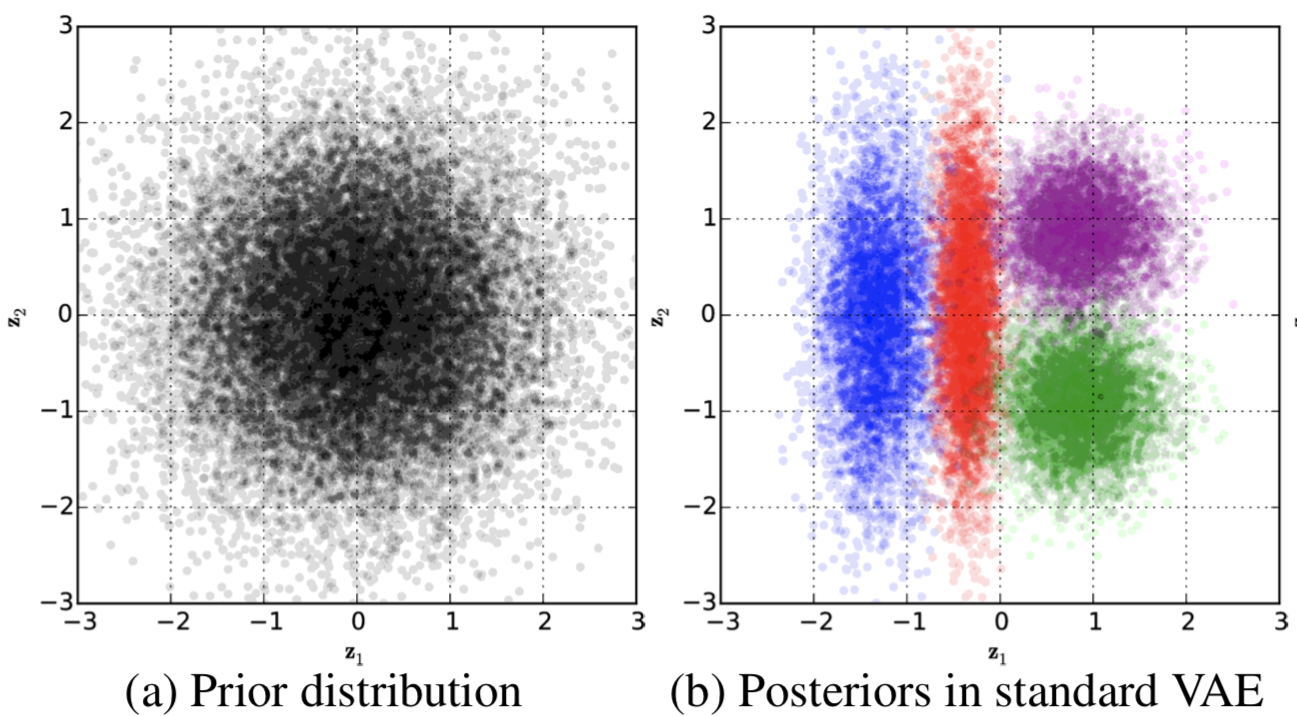
\includegraphics[width=0.7\linewidth]{figs/agg_posterior}
	\end{figure}
\end{frame}
%=======
\begin{frame}{Recap of Previous Lecture}
	\myfootnotewithlink{https://arxiv.org/abs/1711.00937}{Oord A., Vinyals O., Kavukcuoglu K. Neural Discrete Representation Learning, 2017} 
	\begin{block}{Assumptions}
		\begin{itemize}
			\item Let $c \sim \Cat(\bpi)$, where 
			\vspace{-0.6cm}
			\[
				\bpi = (\pi_1, \dots, \pi_K), \quad \pi_k = P(c = k), \quad \sum_{k=1}^K \pi_k = 1.
			\]
			\vspace{-0.7cm}
			\item Suppose the VAE employs a discrete latent code $c$, with prior $p(c) = \Uniform\{1, \dots, K\}$.
		\end{itemize}
	\end{block}
	\vspace{-0.3cm}
	\begin{block}{ELBO}
		\vspace{-0.7cm}
		\[
			\cL_{\bphi, \btheta}(\bx)  = \bbE_{q_{\bphi}(c| \bx)} \log \pt(\bx| c) - {\color{olive} \KL(q_{\bphi}(c| \bx) \,\|\, p(c))} \rightarrow \max_{\bphi, \btheta}.
		\]
	\end{block}
	\vspace{-1.0cm}
	\[
		\KL(q_{\bphi}(c| \bx) \,\|\, p(c)) = - \Ent(q_{\bphi}(c| \bx)) + \log K. 
	\]		
	\vspace{-0.5cm}
	\begin{block}{Vector Quantization}
		Define the codebook $\{\be_k\}_{k=1}^K$, where $\be_k \in \bbR^L$ and $K$ is the size of the dictionary.
		\vspace{-0.3cm}
		\[
			\bz_q = \bq (\bz) = \be_{k^*}, \quad \text{where}\;\; k^* = \argmin_k \| \bz - \be_k \|.
		\] 
		\vspace{-0.7cm}
	\end{block}
\end{frame}
%=======
\begin{frame}{Recap of Previous Lecture}
	\myfootnotewithlink{https://arxiv.org/abs/1711.00937}{Oord A., Vinyals O., Kavukcuoglu K. Neural Discrete Representation Learning, 2017} 
	\begin{figure}
		\centering
		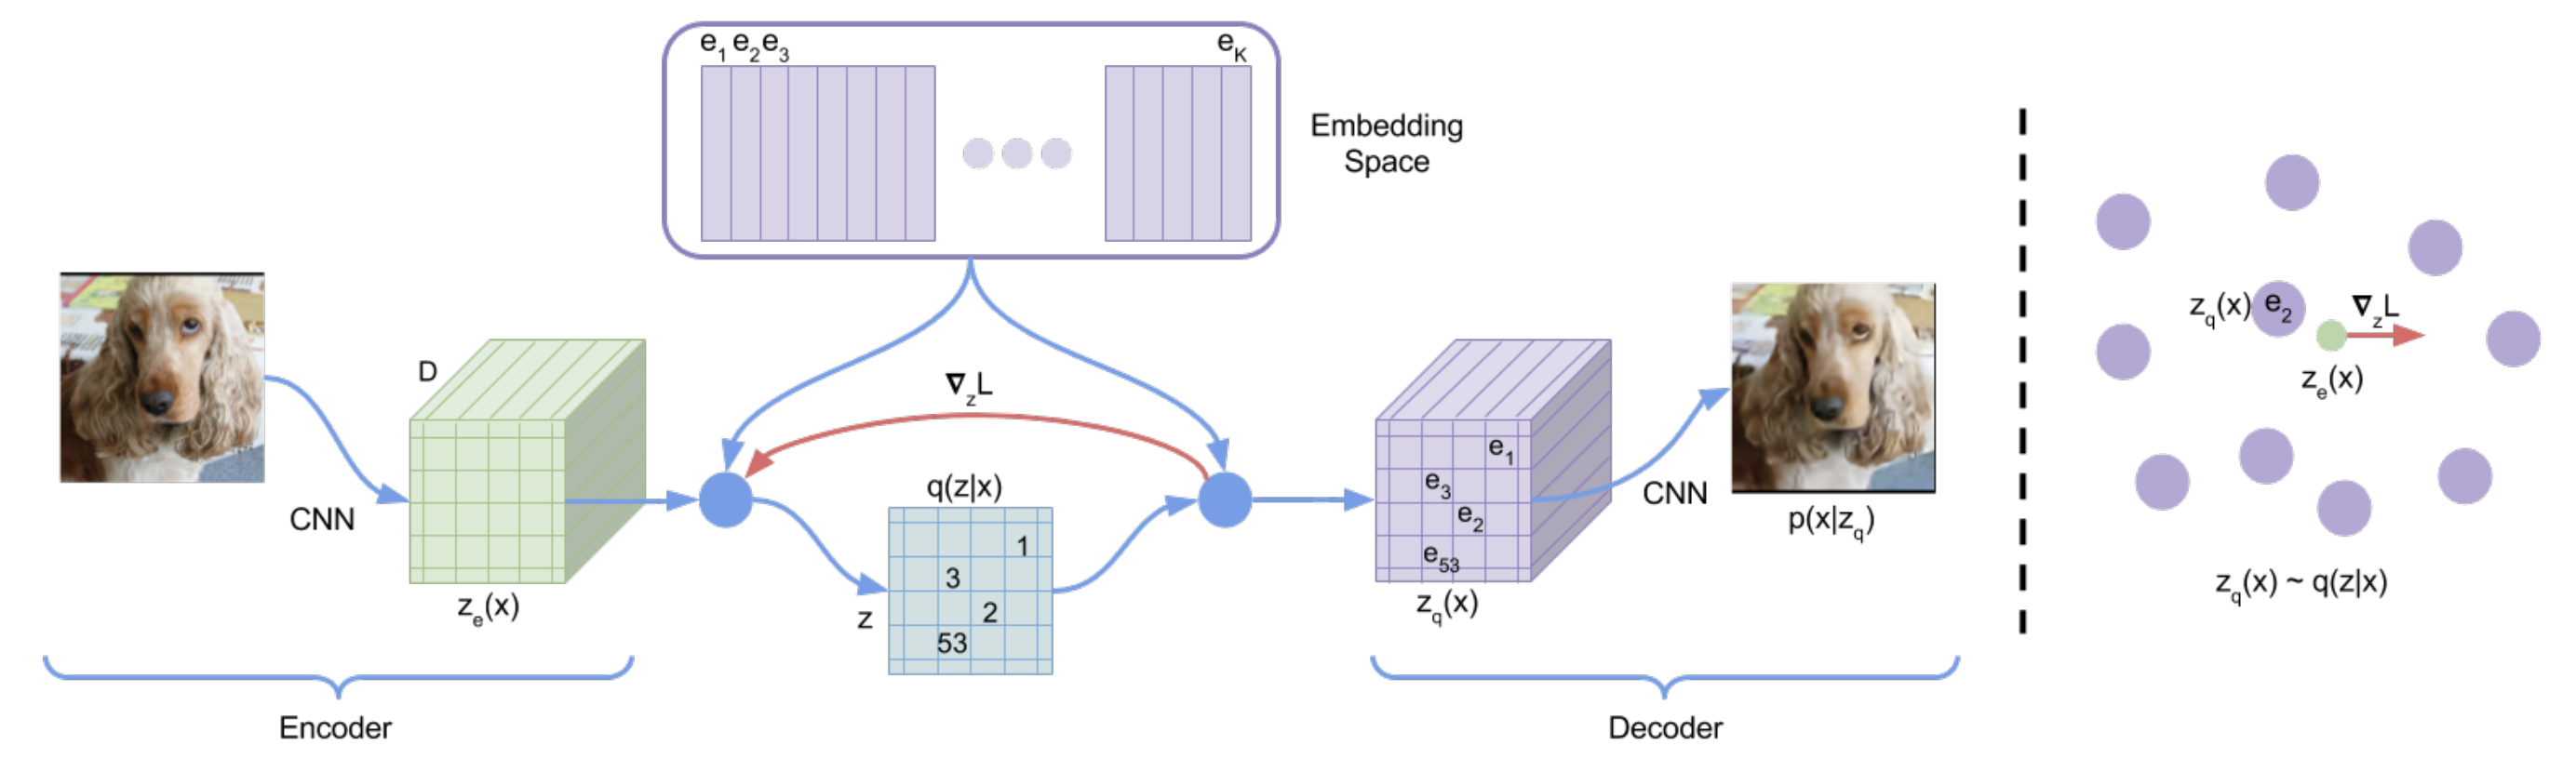
\includegraphics[width=0.85\linewidth]{figs/vqvae}
	\end{figure}
	\vspace{-0.3cm}
	\begin{block}{Deterministic Variational Posterior}
		\vspace{-0.3cm}
		\[
			q_{\bphi}(c_{ij} = k^* | \bx) = \begin{cases}
				1,  & \text{if}\;\; k^* = \argmin_k \| [\bz_e]_{ij} - \be_k \|; \\
				0,  & \text{otherwise}.
			\end{cases}
		\]
		\vspace{-0.5cm}
	\end{block}
	\begin{block}{ELBO}
		\vspace{-0.6cm}
		\[
			\cL_{\bphi, \btheta}(\bx)  = \bbE_{q_{\bphi}(c| \bx)} \log \pt(\bx| \be_{c}) - \log K =  \log \pt(\bx| \bz_q) - \log K.
		\]
		\vspace{-0.6cm}
	\end{block}
	\begin{block}{Straight-Through Gradient Estimation}
		\vspace{-0.6cm}
		\[
			\frac{\partial \log p(\bx | \bz_q , \btheta)}{\partial \bphi} = \frac{\partial \log \pt(\bx| \bz_q)}{\partial \bz_q} \cdot {\color{red}\frac{\partial \bz_q}{\partial \bphi}} \approx \frac{\partial \log \pt(\bx| \bz_q)}{\partial \bz_q} \cdot \frac{\partial \bz_e}{\partial \bphi}
		\]
	\end{block}
\end{frame}
%=======
\begin{frame}{Recap of Previous Lecture}
	\begin{block}{Likelihood-Free Learning}
		\begin{itemize}
			\item Likelihood isn't a perfect metric for generative models.
			\item Likelihood may be intractable.
		\end{itemize}
	\end{block}
	Imagine we have two sets of samples:
	\begin{itemize}
		\item $\{\bx_i\}_{i=1}^{n_1} \sim \pd(\bx)$ -- real samples;
		\item $\{\bx_i\}_{i=1}^{n_2} \sim \pt(\bx)$ -- generated (fake) samples.
	\end{itemize}
	\[
		p(y = 1 | \bx) = P(\bx \sim \pd(\bx)); \quad p(y = 0 | \bx) = P(\bx \sim \pt(\bx))
	\]
	\vspace{-0.5cm}
	\begin{block}{Assumption}
		The generative distribution $\pt(\bx)$ matches the true distribution $\pd(\bx)$ if we can't distinguish between them using a discriminative model $p(y|\bx)$.
	\end{block}
	\begin{itemize}
		\item \textbf{Generator:} a generative model $\bx = \bG(\bz)$ that produces more realistic samples.
		\item \textbf{Discriminator:} a classifier $D(\bx) \in [0, 1]$ distinguishing real from generated samples.
	\end{itemize}
\end{frame}
%=======
\begin{frame}{Outline}
	\tableofcontents
\end{frame}
%=======
\section{Generative Adversarial Networks (GAN)}
%=======
\begin{frame}{Generative Models Taxonomy}
	\renderTaxonomy{gan}
\end{frame}
%=======
\begin{frame}{GAN Optimality}
	\myfootnotewithlink{https://arxiv.org/abs/1406.2661}{Goodfellow I. J. et al. Generative Adversarial Networks, 2014}
	\begin{block}{Theorem}
		The minimax game
		\vspace{-0.3cm}
		\[
			\min_{G} \max_D \Bigl[ \underbrace{\bbE_{\pd(\bx)} \log D(\bx) + \bbE_{p(\bz)} \log (1 - D(\bG(\bz)))}_{V(G, D)} \Bigr]
		\]
		\vspace{-0.5cm} \\
		achieves its global optimum when $\pd(\bx) = \pt(\bx)$, and $D^*(\bx) = 0.5$.
	\end{block}
	\eqpause
	\begin{block}{Proof (Fixed $G$)}
		\vspace{-0.5cm}
		\begin{align*}
			V(G, D) &= \bbE_{\pd(\bx)} \log D(\bx) + \bbE_{\pt(\bx)} \log (1 - D(\bx)) \\
			\nextonslide{&= \int \underbrace{\left[ \pd(\bx) \log D(\bx) + \pt(\bx)\log (1 - D(\bx)) \right]}_{y(D)} d \bx}
		\end{align*}
		\eqpause
		\vspace{-0.2cm}
		\[
			\frac{d y(D)}{d D} = \frac{\pd(\bx)}{D(\bx)} - \frac{\pt(\bx)}{1 - D(\bx)} = 0 \qquad \Rightarrow \quad D^*(\bx) = \frac{\pd(\bx)}{\pd(\bx) + \pt(\bx)}
		\]
	\end{block}
\end{frame}
%=======
\begin{frame}{GAN Optimality}
	\myfootnotewithlink{https://arxiv.org/abs/1406.2661}{Goodfellow I. J. et al. Generative Adversarial Networks, 2014}
	\begin{block}{Proof Continued (Fixed $D = D^*$)}
		\vspace{-0.5cm}
		{\small
		\begin{multline*}
			V(G, D^*) = \bbE_{\pd(\bx)} \log \left( \frac{\pd(\bx)}{\pd(\bx) + \pt(\bx)} \right) + \bbE_{\pt(\bx)} \log \left( \frac{\pt(\bx)}{\pd(\bx) + \pt(\bx)}\right)  \\
		 \nextonslide{= \KL \left(\pd(\bx) \,\|\, \frac{\pd(\bx) + \pt(\bx)}{2}\right) + \KL \left(\pt(\bx) \,\|\, \frac{\pd(\bx) + \pt(\bx)}{2}\right) - 2\log 2 \\}
		 \nextonslide{= 2\,\JSD(\pd(\bx) \,\|\, \pt(\bx)) - 2\log 2.}
		\end{multline*}
		}
	\end{block}
	\eqpause
	\vspace{-0.3cm}
	\begin{block}{Jensen-Shannon Divergence (Symmetric KL Divergence)}
		\vspace{-0.3cm}
		\[
			\JSD(\pd(\bx) \| \pt(\bx)) = \frac{1}{2} \left[\KL \left(\pd(\bx) \| {\color{teal}\star}\right) + \KL \left(\pt(\bx) \| {\color{teal}\star}\right) \right]
		\]
	\end{block}
	\eqpause
	This can be regarded as a proper distance metric!
	\[
		V(G^*, D^*) = -2\log 2, \quad \pd(\bx) = \pt(\bx), \quad  D^*(\bx) = 0.5.
	\]
\end{frame}
%=======
\begin{frame}{GAN Optimality}
	\myfootnotewithlink{https://arxiv.org/abs/1406.2661}{Goodfellow I. J. et al. Generative Adversarial Networks, 2014}
	\begin{block}{Theorem}
		The following minimax game 
		\vspace{-0.3cm}
		\[
		\min_{G} \max_D \Bigl[ \bbE_{\pd(\bx)} \log D(\bx) + \bbE_{p(\bz)} \log (1 - D(\bG(\bz))) \Bigr]
		\]
		\vspace{-0.5cm} \\
		achieves its global optimum precisely when $\pd(\bx) = \pt(\bx)$, and $D^*(\bx) = 0.5$.
	\end{block}
	\vspace{-0.2cm}
	\begin{block}{Expectations}
		If the generator can express \textbf{any} function and the discriminator is \textbf{optimal} at every step, the generator \textbf{will converge} to the target distribution.
	\end{block}
	\vspace{-0.3cm}
	\eqpause
	\begin{block}{Reality}
		\begin{itemize}
			\item Generator updates are performed in parameter space, and the discriminator is often imperfectly optimized.
			\item Generator and discriminator losses typically oscillate during GAN training.
		\end{itemize}
	\end{block}
\end{frame}
%=======
\begin{frame}{GAN Training}
	\myfootnotewithlink{https://arxiv.org/abs/1406.2661}{Goodfellow I. J. et al. Generative Adversarial Networks, 2014}

	Assume both generator and discriminator are parametric models: $D_{\bphi}(\bx)$ and $\bG_{\btheta}(\bz)$.
	\begin{block}{Objective}
		\vspace{-0.7cm}
		\[
		\min_{\btheta} \max_{\bphi} \left[ \bbE_{\pd(\bx)} \log D_{\bphi}(\bx) + \bbE_{p(\bz)} \log (1 - D_{\bphi}(\bG_{\btheta}(\bz))) \right]
		\]
		\vspace{-0.7cm}
	\end{block}
	\eqpause
	\begin{figure}
		\centering
		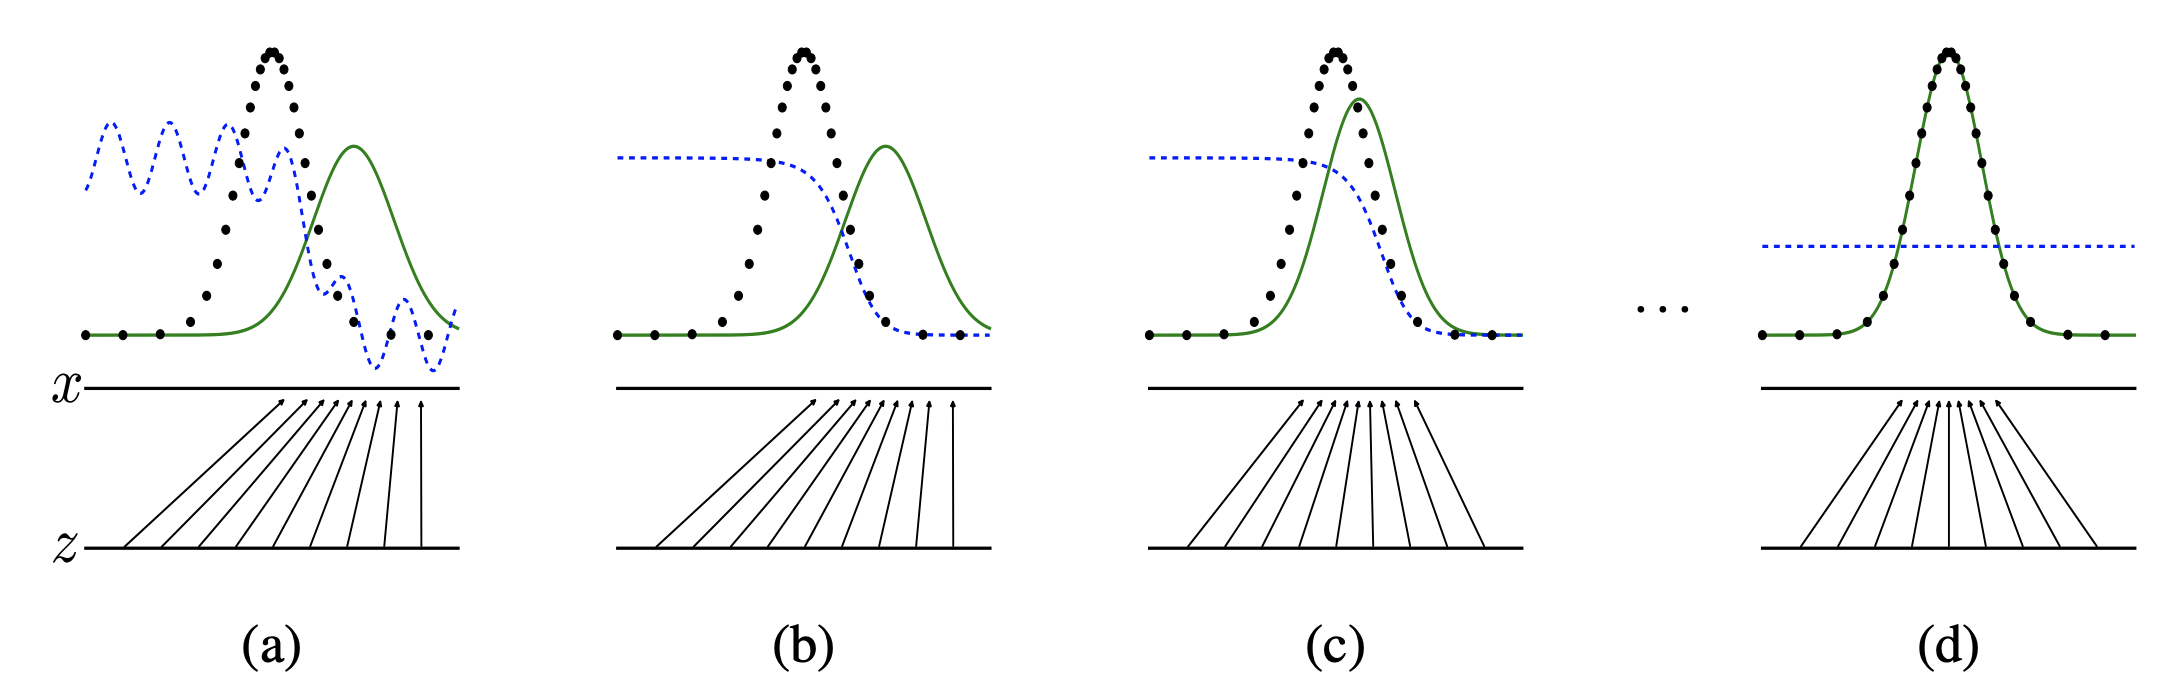
\includegraphics[width=1.0\linewidth]{figs/gan_1}
	\end{figure}
	\vspace{-0.5cm}
	\eqpause
	\begin{itemize}
		\item $\bz \sim p(\bz)$ is a latent variable.
		\item $\pt(\bx | \bz) = \delta(\bx - \bG_{\btheta}(\bz))$ serves as a deterministic decoder ({\color{gray}like normalizing flows}).
		\item There is no encoder present.
	\end{itemize}
\end{frame}
%=======
\begin{frame}{Mode Collapse}
	\myfootnote{\href{https://arxiv.org/abs/1406.2661}{Goodfellow I. J. et al. Generative Adversarial Networks, 2014} \\
		\href{https://arxiv.org/abs/1611.02163}{Metz L. et al. Unrolled Generative Adversarial Networks, 2016}}
	Mode collapse refers to the phenomenon where the generator in a GAN produces only one or a few different modes of the distribution.
	\vspace{-0.1cm}
	\begin{figure}
		\centering
		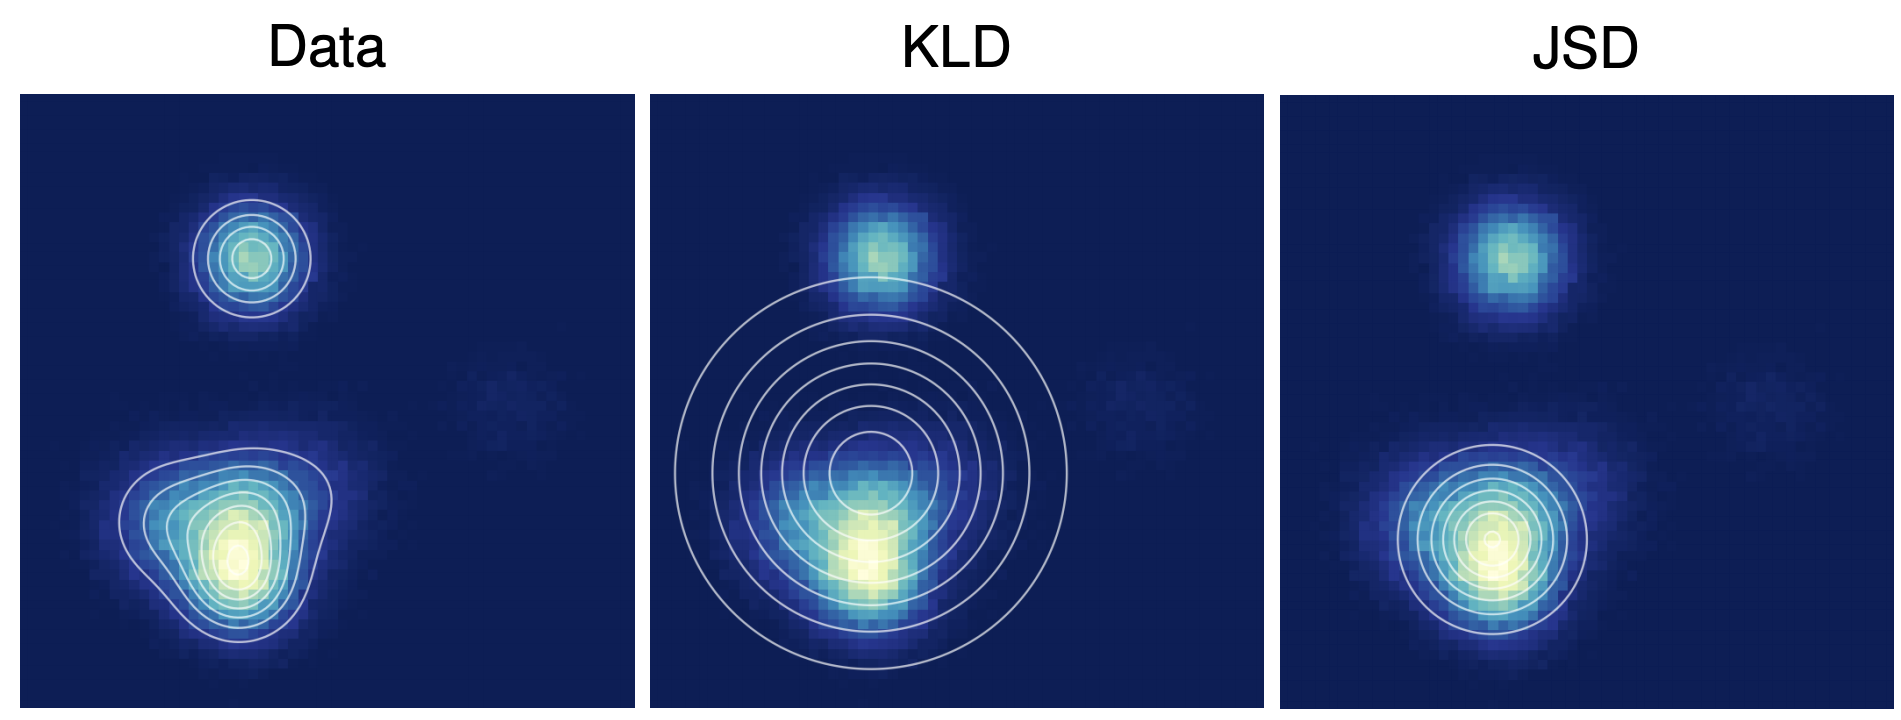
\includegraphics[width=0.75\linewidth]{figs/mode_collapse_1}
	\end{figure}
	\vspace{-0.3cm}
	\begin{figure}
		\centering
		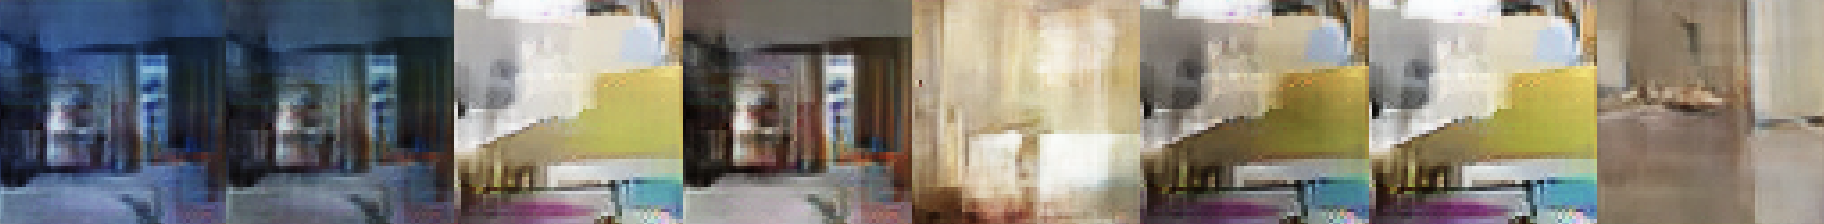
\includegraphics[width=1.0\linewidth]{figs/mode_collapse_4}
	\end{figure}
	\eqpause
	Numerous methods have been proposed to tackle mode collapse: changing architectures, adding regularization terms, injecting noise.
\end{frame}
%=======
\begin{frame}{Jensen-Shannon vs Kullback-Leibler Divergences}
	\begin{itemize}
		\item $\pd(\bx)$ is a fixed mixture of two Gaussians.
		\item $p(\bx | \mu, \sigma) = \cN(\mu, \sigma^2)$.
	\end{itemize}
	\begin{block}{Mode Covering vs. Mode Seeking}
		\vspace{-0.7cm}
		\[
			\KL(\pi \,\|\, p) = \int \pi(\bx) \log \frac{\pi(\bx)}{p(\bx)}d\bx, 
			\quad \KL(p \| \pi) = \int p(\bx) \log \frac{p(\bx)}{\pi(\bx)}d\bx
		\]
		\[
			\JSD(\pi \,\|\, p) = \frac{1}{2} \Bigl[\KL \Bigl(\pi(\bx) \,\|\, \frac{\pi(\bx) + p(\bx)}{2}\Bigr) + \KL \Bigl(p(\bx) \,\|\, \frac{\pi(\bx) + p(\bx)}{2}\Bigr) \Bigr]
		\]
		\vspace{-0.7cm}
		\eqpause
		\begin{minipage}[t]{0.33\columnwidth}
			\begin{figure}
				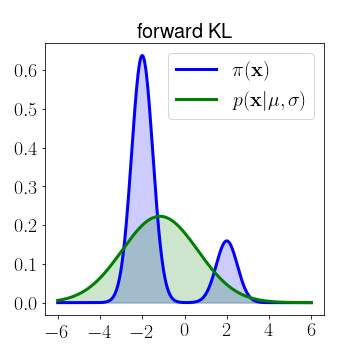
\includegraphics[width=\linewidth]{figs/forward_KL}
			\end{figure}
		\end{minipage}%
		\begin{minipage}[t]{0.33\columnwidth}
			\begin{figure}
				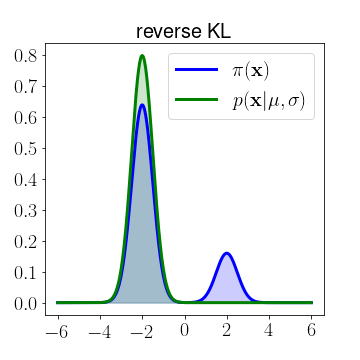
\includegraphics[width=\linewidth]{figs/reverse_KL}
			\end{figure}
		\end{minipage}%
		\begin{minipage}[t]{0.33\columnwidth}
			\begin{figure}
				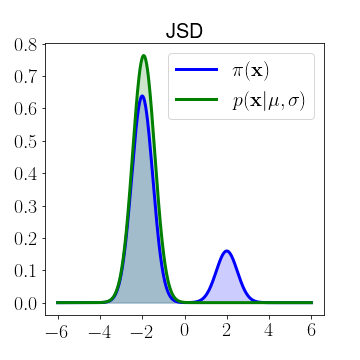
\includegraphics[width=\linewidth]{figs/JSD}
			\end{figure}
		\end{minipage}
		\vspace{-0.3cm}
	\end{block}
\end{frame}
%=======
\section{Wasserstein Distance}
%=======
\begin{frame}{Theoretical Results}
	\myfootnote{\href{https://arxiv.org/abs/1904.08994}{Weng L. From GAN to WGAN, 2019} \\ 
		\href{https://arxiv.org/abs/1701.04862}{Arjovsky M., Bottou L. Towards Principled Methods for Training Generative Adversarial Networks, 2017}}
	\vspace{-0.3cm}
	\begin{itemize}
		\item The dimensionality of $\bz$ is less than that of $\bx$, so $\pt(\bx)$ with $\bx = \bG_{\btheta}(\bz)$ lives on a low-dimensional manifold.
		\eqpause
		\item The true data distribution $\pd(\bx)$ is also supported on a low-dimensional manifold.
		\begin{figure}
			\centering
			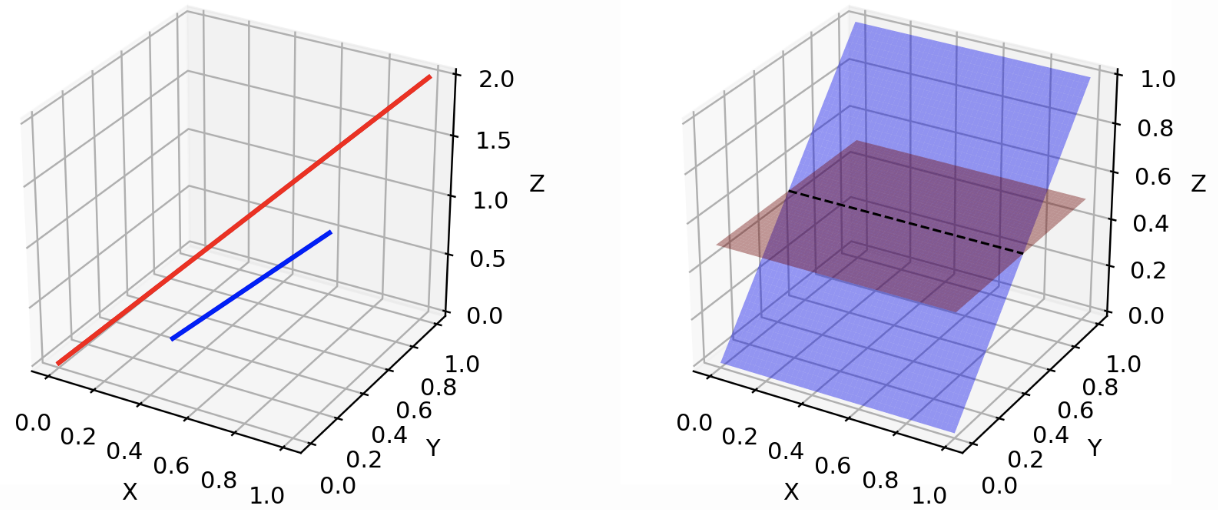
\includegraphics[width=0.55\linewidth]{figs/low_dim_manifold}
		\end{figure}
		\eqpause
		\item If $\pd(\bx)$ and $\pt(\bx)$ are disjoint, a smooth optimal discriminator can exist!
		\eqpause
		\item For such low-dimensional, disjoint manifolds:
		\vspace{-0.2cm}
		\[
			\KL(\pd\,\|\,\pt) = \KL(\pt\,\|\,\pd) = \infty, \quad \JSD(\pd\,\|\,\pt) = \log 2
		\]
	\end{itemize}
\end{frame}
%=======
\begin{frame}{Wasserstein Distance (Discrete)}
	\myfootnotewithlink{https://udlbook.github.io/udlbook/}{Simon J.D. Prince. Understanding Deep Learning, 2023}
	Also known as the \textbf{Earth Mover's Distance}.
	\begin{block}{Optimal Transport Formulation}
		The minimum cost of moving and transforming a pile of ``dirt'' shaped like one probability distribution to match another.
	\end{block}
	\begin{figure}
		\centering
		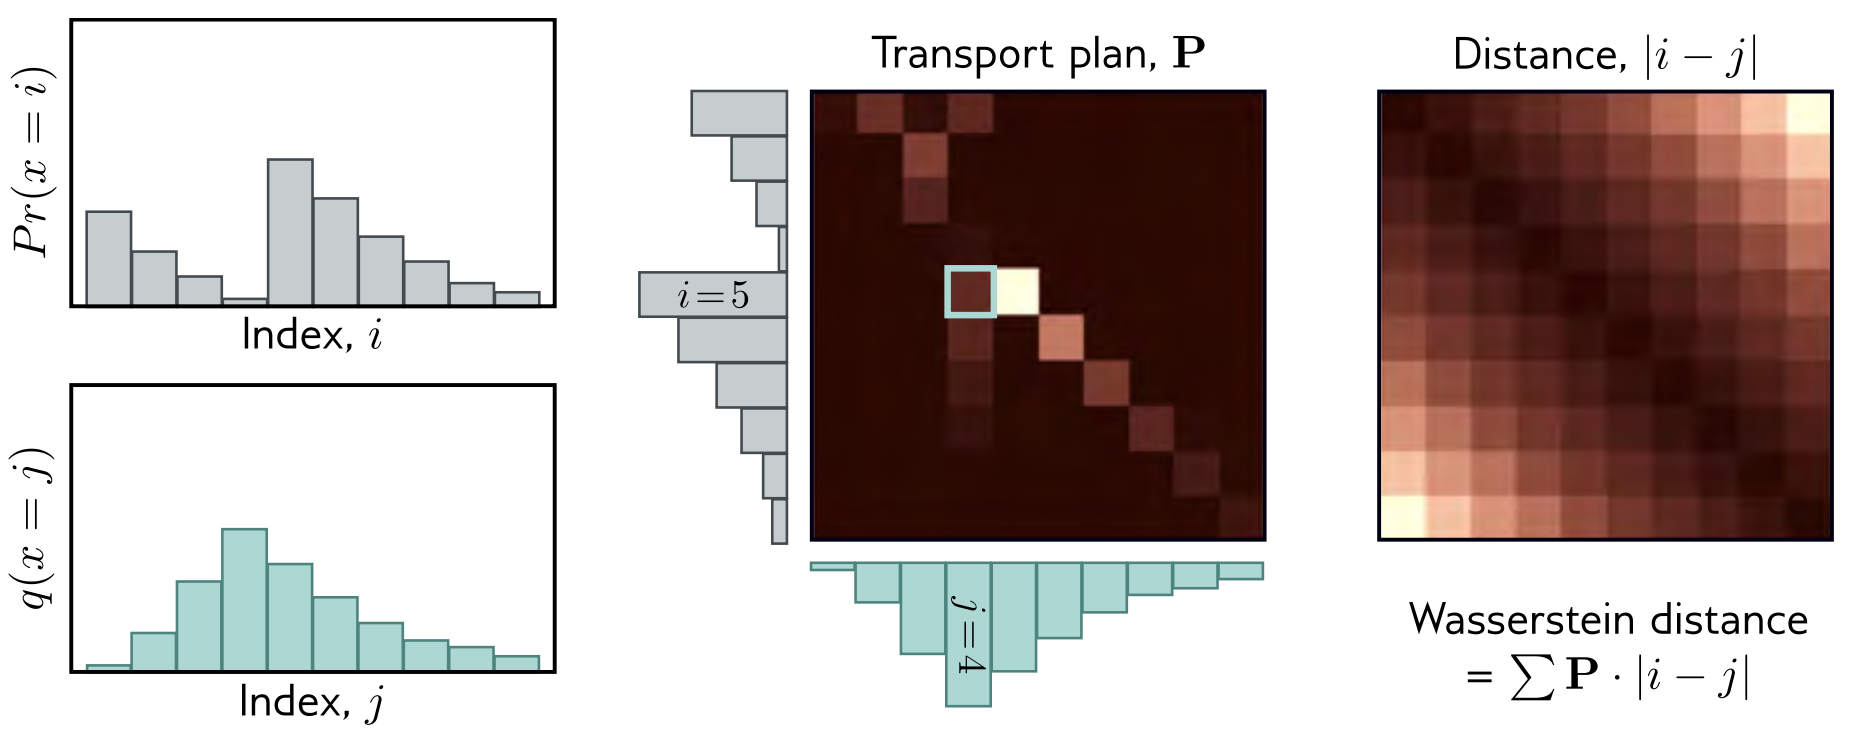
\includegraphics[width=\linewidth]{figs/discrete_wasserstein}
	\end{figure}
\end{frame}
%=======
\begin{frame}{Wasserstein Distance (Continuous)}
	\myfootnotewithlink{https://arxiv.org/abs/1701.07875}{Arjovsky M., Chintala S., Bottou L. Wasserstein GAN, 2017}
	\vspace{-0.5cm}
	{
	\small
	\[
		W(\pi \| p) = \inf_{\gamma \in \Gamma(\pi, p)} \bbE_{(\bx_1, \bx_2) \sim \gamma} \| \bx_1 - \bx_2 \| =  \inf_{{\color{olive}\gamma} \in {\color{teal}\Gamma(\pi, p)}} \int {\color{violet} \| \bx_1 - \bx_2 \|}\, {\color{olive}\gamma (\bx_1, \bx_2)} d \bx_1 d \bx_2
	\]
	}
	\vspace{-0.4cm}
	\begin{itemize}
		\item ${\color{olive}\gamma (\bx_1, \bx_2)}$ is the transport plan: the amount of “dirt” assigned from $\bx_1$ to $\bx_2$.
		\vspace{-0.2cm}
		\[
		\int \gamma(\bx_1, \bx_2) d \bx_1 = p(\bx_2); \quad \int \gamma(\bx_1, \bx_2) d \bx_2 = \pi(\bx_1).
		\]
		\vspace{-0.6cm}
		\item ${\color{teal}\Gamma(\pi, p)}$ denotes the set of all joint distributions $\gamma (\bx_1, \bx_2)$ with marginals $\pi$ and $p$.
		\item ${\color{olive}\gamma(\bx_1, \bx_2)}$ is the mass, ${\color{violet}\|\bx_1 - \bx_2\|}$ is the distance.
	\end{itemize}
	\eqpause
	\begin{block}{Wasserstein Metric}
		\vspace{-0.2cm}
		\[
		W_s(\pi, p) = \inf_{\gamma \in \Gamma(\pi, p)} \Bigl(\bbE_{(\bx_1, \bx_2) \sim \gamma} \|\bx_1 - \bx_2\|^s\Bigr)^{1/s}
		\]
		\vspace{-0.4cm}
	\end{block}
	In our setting, $W(\pi \| p) = W_1(\pi, p)$, which is the transport cost formulation.
\end{frame}
%=======
\begin{frame}{Wasserstein Distance vs KL vs JSD}
	\myfootnote{\href{https://arxiv.org/abs/1904.08994}{Weng L. From GAN to WGAN, 2019} \\ 
		\href{https://arxiv.org/abs/1701.07875}{Arjovsky M., Chintala S., Bottou L. Wasserstein GAN, 2017}}
	\begin{minipage}[t]{0.48\columnwidth}
		Consider two-dimensional distributions:
		\vspace{-0.3cm}
		\[
			\pd(x, y) = (0, U[0, 1])
		\]	
		\[
			\pt(x, y) = (\theta, U[0, 1])
		\]
	\end{minipage}%
	\begin{minipage}[t]{0.52\columnwidth}
		\vspace{-0.3cm}
		\begin{figure}
			\centering
			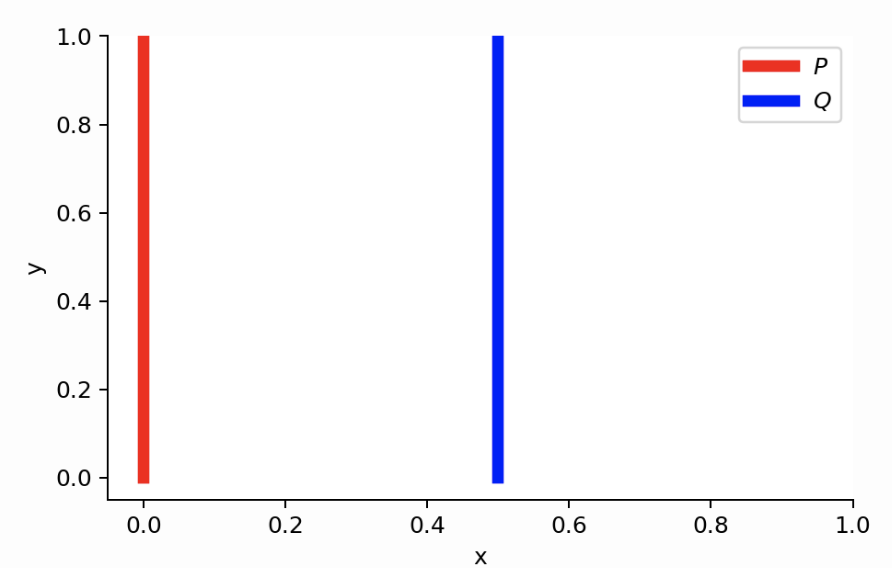
\includegraphics[width=0.8\linewidth]{figs/w_kl_jsd}
		\end{figure}
	\end{minipage}
	\vspace{-0.3cm}
	\eqpause
	\begin{itemize}
		\footnotesize
		\item $\theta = 0$: Both distributions are identical.
		\[
			\KL(\pd \| \pt) = \KL(\pt \| \pd) = \JSD(\pt \| \pd) = W(\pd \| \pt) = 0
		\]
		\vspace{-0.5cm}
		\eqpause
		\item $\theta \neq 0$:
		\vspace{-0.3cm}
		\[
			\KL(\pd \| \pt) = \int_{U[0, 1]} 1 \log \frac{1}{0}\,dy = \infty = \KL(\pt \| \pd)
		\]
		\eqpause
		\[
			\JSD(\pd \| \pt) = \frac{1}{2}\left( \int_{U[0, 1]}1 \log \frac{1}{1/2} dy + \int_{U[0, 1]}1 \log \frac{1}{1/2} dy \right) = \log 2
		\]
		\eqpause
		\[
			W(\pd \| \pt) = |\theta|
		\]
	\end{itemize}
\end{frame}
%=======
\begin{frame}{Wasserstein Distance vs KL vs JSD}
	\myfootnotewithlink{https://arxiv.org/abs/1701.07875}{Arjovsky M., Chintala S., Bottou L. Wasserstein GAN, 2017}
	\begin{block}{Theorem 1}
		Let $\bG_{\btheta}(\bz)$ be (almost) any feedforward neural network, and $p(\bz)$ a prior over $\bz$ such that $\bbE_{p(\bz)} \|\bz\| < \infty$. Then $W(\pd \| \pt)$ is continuous everywhere and differentiable almost everywhere.
	\end{block}
	\eqpause
	\begin{block}{Theorem 2}
		Let $\pi$ be a distribution on a compact space $\cX$ and let $\{p_t\}_{t=1}^\infty$ be a sequence of distributions on $\cX$. 
		\begin{align}
			\KL(\pi \| p_t) &\rightarrow 0 \ \ (\text{or }\KL (p_t\,\|\,\pi) \rightarrow 0) \\
			\JSD(\pi \| p_t) &\rightarrow 0 \\
			W(\pi \| p_t) &\rightarrow 0
		\end{align}
		As $t \rightarrow \infty$, (1) $\Rightarrow$ (2), and (2) $\Rightarrow$ (3). That is, convergence in Wasserstein distance is a weaker condition than convergence in JSD, which in turn is weaker than convergence in KL.
	\end{block}
\end{frame}
%=======
\section{Wasserstein GAN (WGAN)}
%=======
\begin{frame}{Wasserstein GAN}
	\myfootnotewithlink{https://arxiv.org/abs/1701.07875}{Arjovsky M., Chintala S., Bottou L. Wasserstein GAN, 2017}
	\begin{block}{Wasserstein Distance}
		\vspace{-0.5cm}
		\small
		\[
		W(\pi \| p) = \inf_{\gamma \in \Gamma(\pi, p)} \bbE_{(\bx_1, \bx_2) \sim \gamma} \| \bx_1 - \bx_2 \| =  \inf_{\gamma \in \Gamma(\pi, p)} \int \|\bx_1 - \bx_2\| \gamma (\bx_1, \bx_2)\, d\bx_1\, d\bx_2
		\]
		\vspace{-0.3cm}
	\end{block}
	\eqpause
	The infimum over all possible $\gamma \in \Gamma(\pi, p)$ is computationally intractable.
	\eqpause
	\begin{block}{Theorem (Kantorovich-Rubinstein Duality)}
		\vspace{-0.3cm}
		\[
			W(\pi \| p) = \frac{1}{K} \max_{\| f \|_L \leq K} \Bigl[ \bbE_{\pi(\bx)} f(\bx)  - \bbE_{p(\bx)} f(\bx)\Bigr]
		\]
		where $f : \bbR^m \rightarrow \bbR$ is $K$-Lipschitz ($\|f\|_L \leq K$):
		\[
			|f(\bx_1) - f(\bx_2)| \leq K \|\bx_1 - \bx_2\|,\quad \forall\ \bx_1, \bx_2 \in \cX.
		\]
		\vspace{-0.6cm}
	\end{block}
	\eqpause
	We can thus estimate $W(\pi \| p)$ using only samples and a function~$f$.
\end{frame}
%=======
\begin{frame}{Wasserstein GAN}
	\myfootnotewithlink{https://arxiv.org/abs/1701.07875}{Arjovsky M., Chintala S., Bottou L. Wasserstein GAN, 2017}
	\begin{block}{Theorem (Kantorovich-Rubinstein Duality)}
		\[
		W(\pd \| \pt) = \frac{1}{K} \max_{\| f \|_L \leq K} \Bigl[ \bbE_{\pd(\bx)} f(\bx)  - \bbE_{\pt(\bx)} f(\bx)\Bigr]
		\]
	\end{block}
	\begin{itemize}
		\item We must ensure that $f$ is $K$-Lipschitz continuous.
		\item Let $f_{\bphi}(\bx)$ be a feedforward neural network parameterized by $\bphi$.
		\item If the weights $\bphi$ are restricted to a compact set $\bPhi$, then $f_{\bphi}$ is $K$-Lipschitz.
		\eqpause
		\item Clamp weights within the box $\bPhi = [-c, c]^d$ (e.g.\ $c = 0.01$) after each update.
	\end{itemize}
	\begin{multline*}
		K \cdot W(\pd \| \pt) = \max_{\| f \|_L \leq K} \Bigl[ \bbE_{\pd(\bx)} f(\bx)  - \bbE_{\pt(\bx)} f(\bx)\Bigr]\ \geq\ 
		\\  \geq \max_{\bphi \in \bPhi} \Bigl[ \bbE_{\pd(\bx)} f_{\bphi}(\bx)  - \bbE_{\pt(\bx)} f_{\bphi}(\bx)\Bigr]
	\end{multline*}
\end{frame}
%=======
\begin{frame}{Wasserstein GAN}
	\myfootnotewithlink{https://arxiv.org/abs/1701.07875}{Arjovsky M., Chintala S., Bottou L. Wasserstein GAN, 2017}
	\begin{block}{Standard GAN Objective}
		\vspace{-0.2cm}
		\[
			\min_{\btheta} \max_{\bphi} \bbE_{\pd(\bx)} \log D_{\bphi}(\bx) + \bbE_{p(\bz)} \log (1 - D_{\bphi}(\bG_{\btheta}(\bz)))
		\]
		\vspace{-0.3cm}
	\end{block}
	\begin{block}{WGAN Objective}
		\vspace{-0.3cm}
		\[
			\min_{\btheta} {\color{violet}W(\pd \| \pt)} \approx \min_{\btheta} {\color{violet}\max_{\bphi \in \bPhi} \Bigl[ \bbE_{\pd(\bx)} f_{\bphi}(\bx)  - \bbE_{p(\bz)} f_{\bphi}(\bG_{\btheta}(\bz))\Bigr]}
		\]
		\vspace{-0.3cm}
	\end{block}
	\eqpause
	\begin{itemize}
		\item The discriminator $D$ is replaced by function $f$: in WGAN, it is known as the \textbf{critic}, which is \emph{not} a classifier.
		\item \textit{``Weight clipping is a clearly terrible way to enforce a Lipschitz constraint.''}
		\begin{itemize}
			\item If $c$ is large, optimizing the critic is hard.
			\item If $c$ is small, gradients may vanish.
		\end{itemize}
	\end{itemize}	
\end{frame}
%=======
\begin{frame}{Wasserstein GAN}
	\myfootnotewithlink{https://arxiv.org/abs/1701.07875}{Arjovsky M., Chintala S., Bottou L. Wasserstein GAN, 2017}
	\vspace{-0.3cm}
	
	\begin{minipage}[t]{0.6\columnwidth}
		\begin{itemize}
			\item WGAN provides nonzero gradients even if distributions' supports are disjoint.
			\item $\JSD(\pd \| \pt)$ is poorly correlated with sample quality and remains near its maximum value $\log 2 \approx 0.69$.
			\item $W(\pd \| \pt)$ is tightly correlated with quality.
		\end{itemize}
	\end{minipage}%
	\begin{minipage}[t]{0.4\columnwidth}
		\begin{figure}
			\centering
			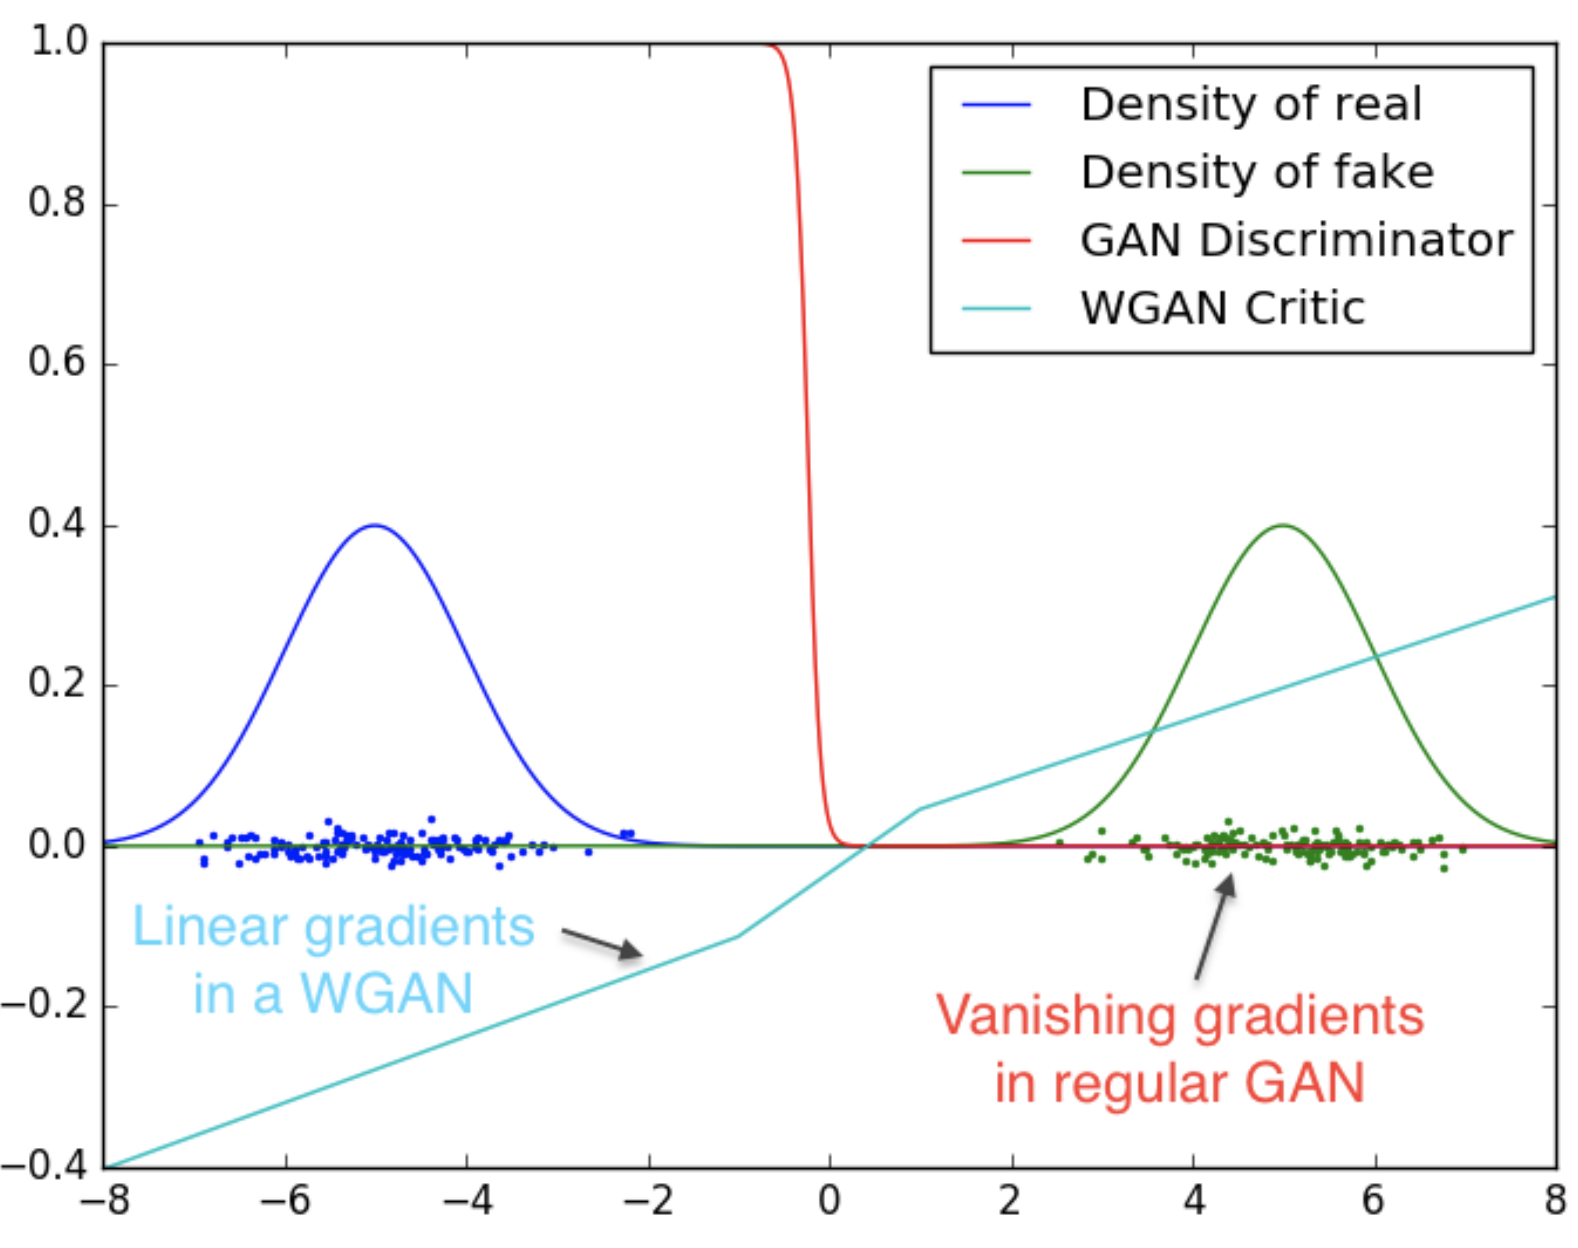
\includegraphics[width=\linewidth]{figs/wgan_toy}
		\end{figure}
	\end{minipage}
	\begin{minipage}[t]{0.5\columnwidth}
		\begin{figure}
			\centering
			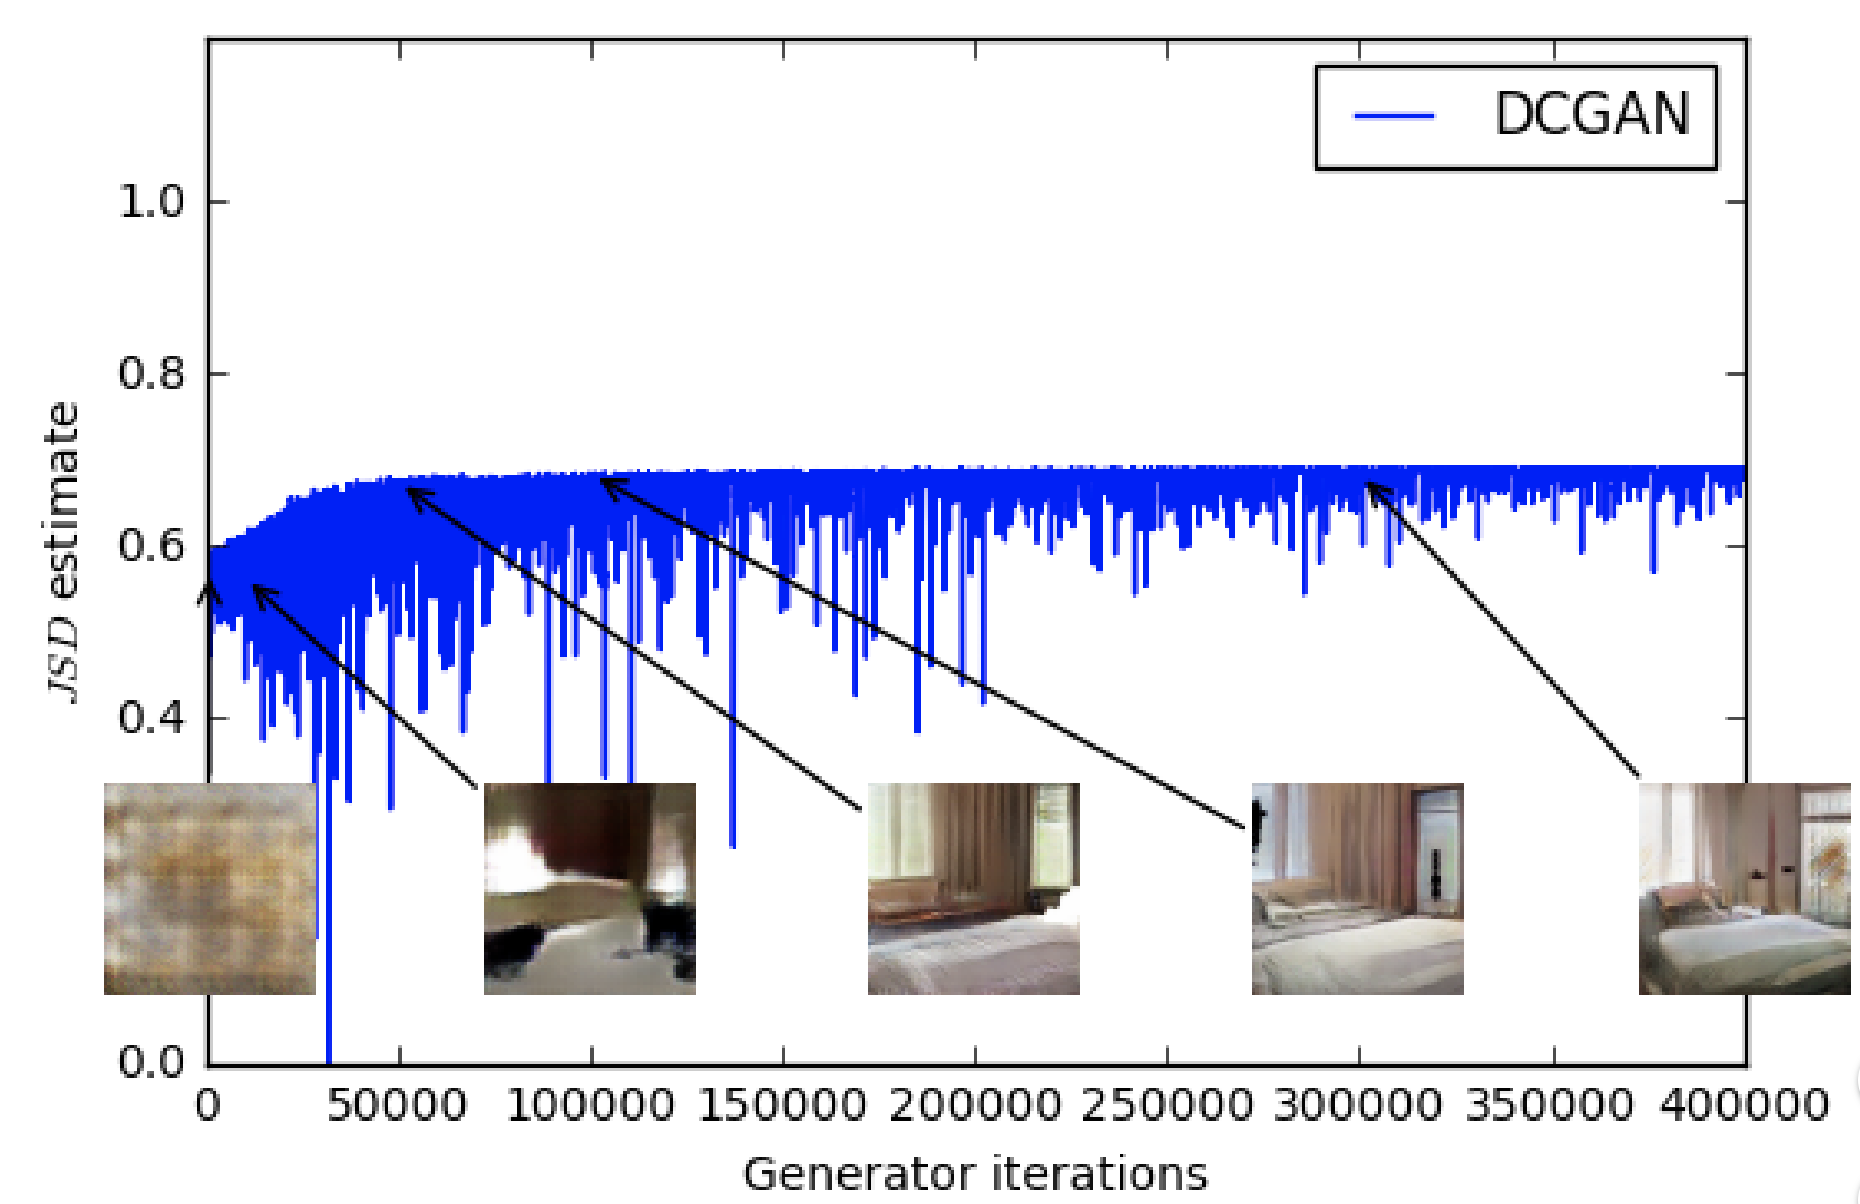
\includegraphics[width=0.95\linewidth]{figs/dcgan_quality}
		\end{figure}
	\end{minipage}%
	\begin{minipage}[t]{0.5\columnwidth}
		\begin{figure}
			\centering
			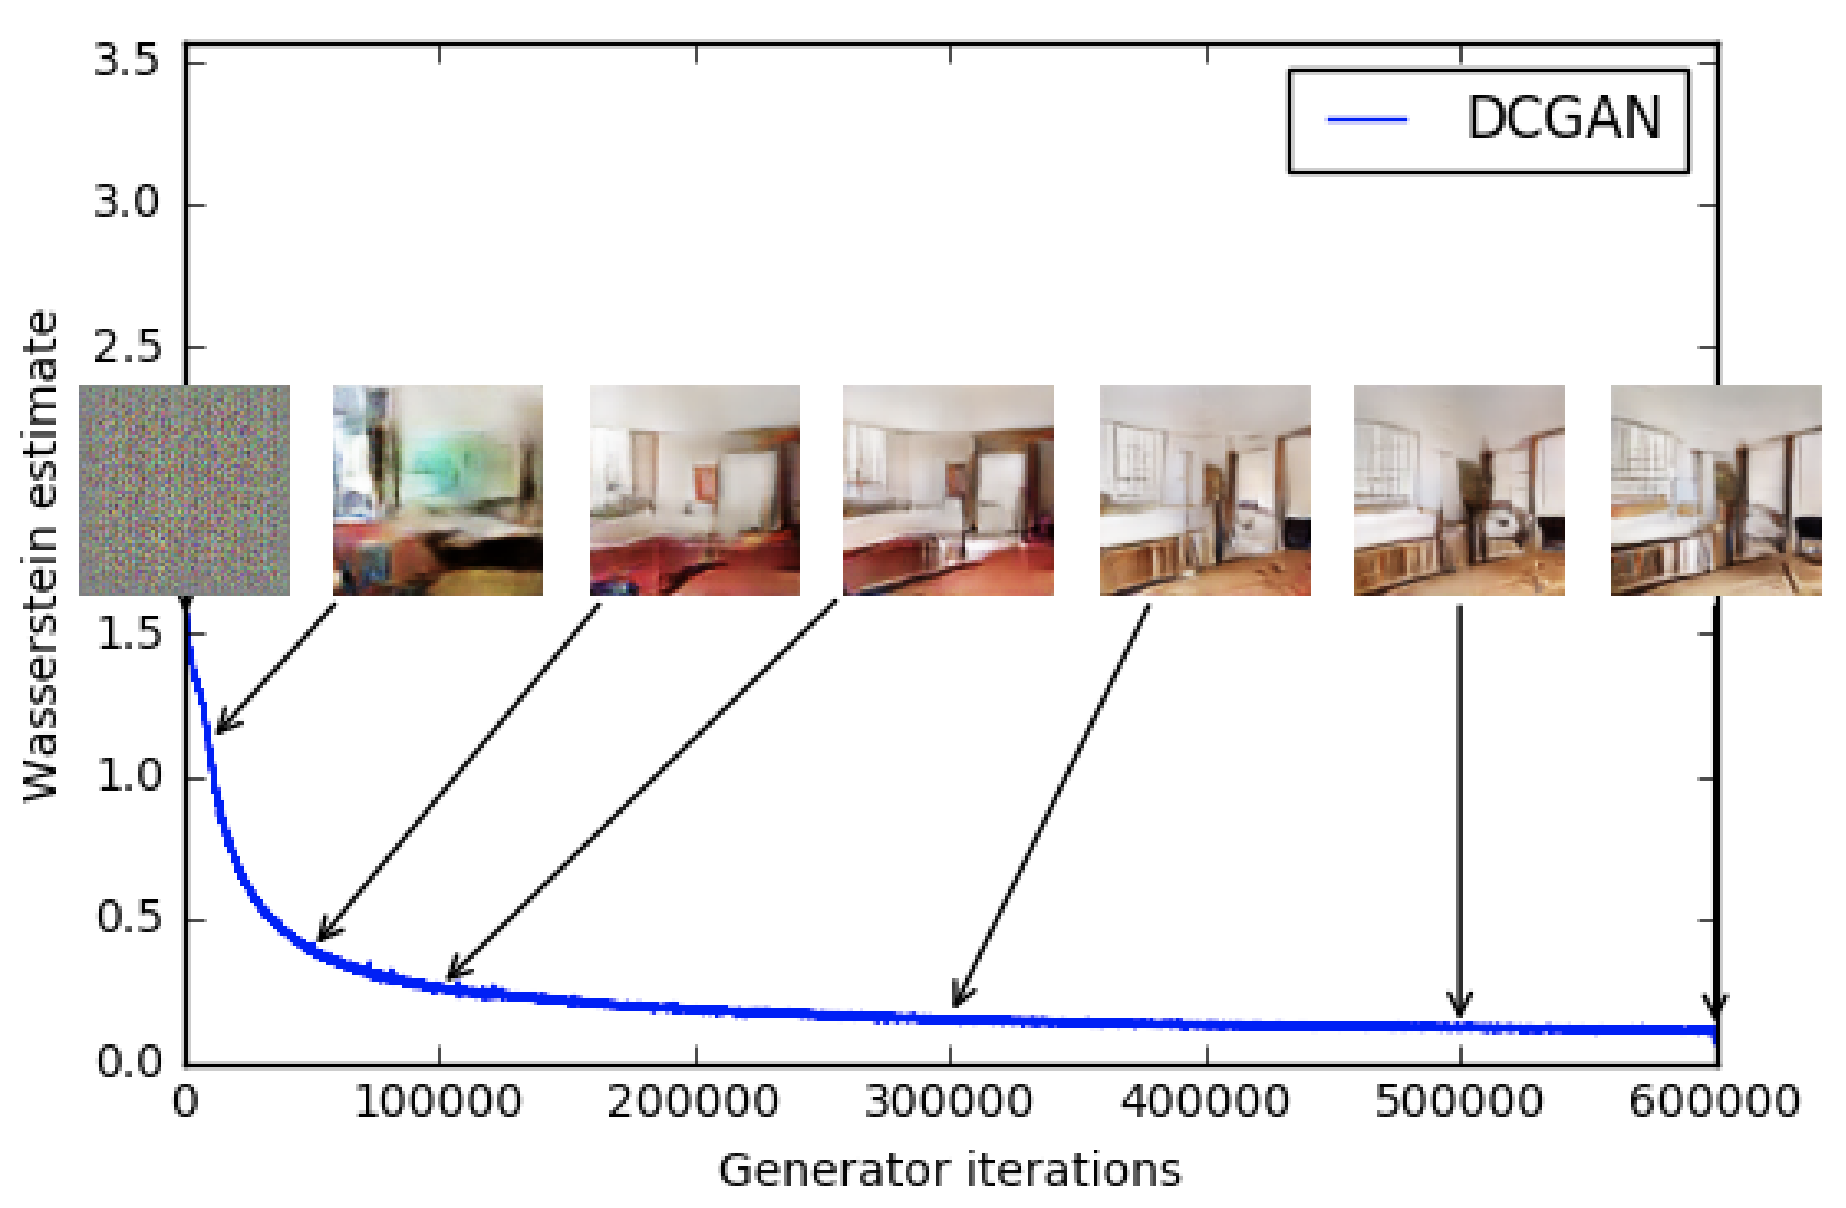
\includegraphics[width=0.95\linewidth]{figs/wgan_quality}
		\end{figure}
	\end{minipage}
\end{frame}
%=======
\section{Evaluation of Likelihood-Free Models}
%=======
\begin{frame}{Evaluation of Likelihood-Free Models}
\myfootnotewithlink{https://deepgenerativemodels.github.io}{image credit: https://deepgenerativemodels.github.io}
	\begin{block}{Likelihood-Based Models}
		\begin{itemize}
			\item \textbf{Train:} fit the model.
			\item \textbf{Validation:} tune hyperparameters.
			\item \textbf{Test:} assess generalization by reporting likelihood.
		\end{itemize}
	\end{block}
	\eqpause
	Not all models have tractable likelihoods \\ (VAE: compare ELBO values; GAN: \textbf{???}).
	\eqpause
	\begin{block}{Desirable Properties for Samples}
		\begin{itemize}
			\item Sharpness
			\begin{figure}
				\centering
				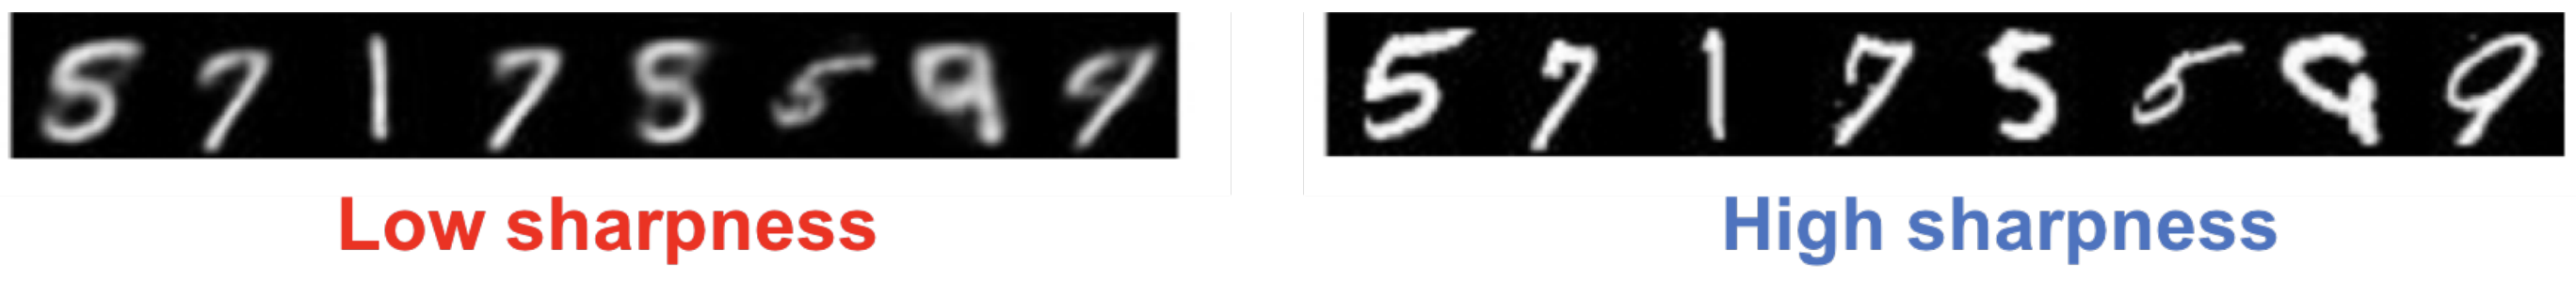
\includegraphics[width=0.9\linewidth]{figs/sharpness}
			\end{figure}
			\eqpause
			\item Diversity
			\begin{figure}
				\centering
				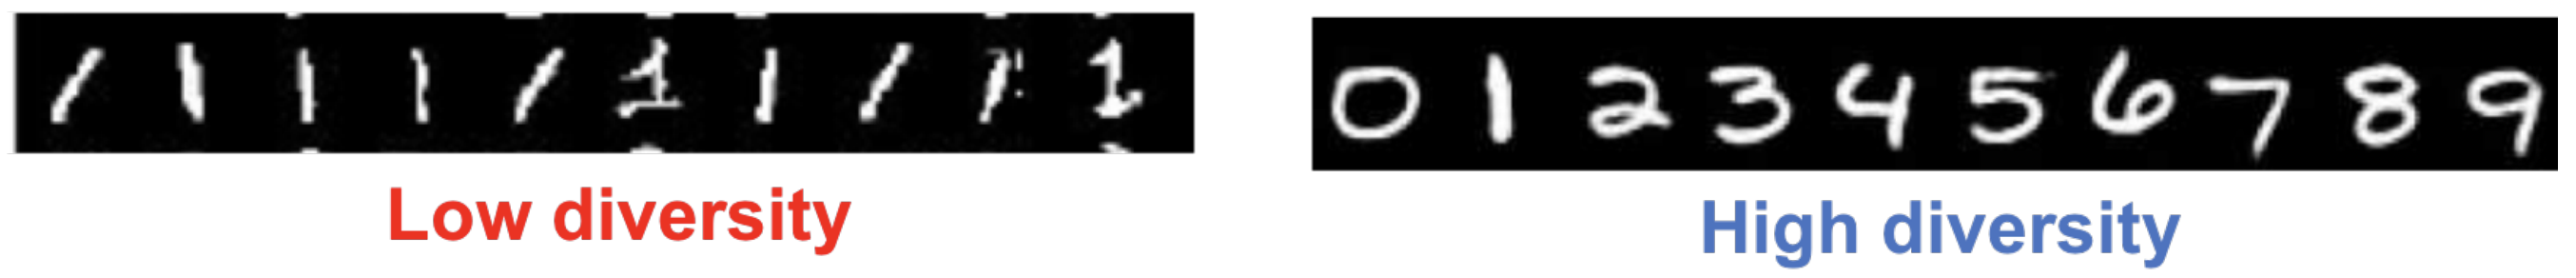
\includegraphics[width=0.9\linewidth]{figs/diversity}
			\end{figure}
		\end{itemize}
	\end{block}
\end{frame}
%=======
\subsection{Frechet Inception Distance (FID)}
%=======
\begin{frame}{Wasserstein Metric}
	\myfootnotewithlink{https://arxiv.org/abs/1706.08500}{Heusel M. et al. GANs Trained by a Two Time-Scale Update Rule Converge to a Local Nash Equilibrium, 2017}
	\vspace{-0.2cm}
	\[
		W_s(\pi \| p) = \inf_{\gamma \in \Gamma(\pi, p)} \left(\bbE_{(\bx_1, \bx_2) \sim \gamma} \| \bx_1 - \bx_2 \|^s\right)^{1/s}
	\]
	\eqpause
	\vspace{-0.3cm}
	\begin{block}{Wasserstein GAN (Optimal Transport)}
		\vspace{-0.5cm}
		{\small
		\[
			W(\pi \| p) = \inf_{\gamma \in \Gamma(\pi, p)} \bbE_{(\bx_1, \bx_2) \sim \gamma} \| \bx_1 - \bx_2 \| =  \inf_{\gamma\in {\Gamma(\pi, p)}} \int { \| \bx_1 - \bx_2 \|} {\gamma (\bx_1, \bx_2)} d \bx_1 d \bx_2
		\]
		}
		\vspace{-0.5cm}
	\end{block}
	\eqpause
	\begin{block}{Theorem}
		If $\pi(\bx) = \cN(\bmu_\pi, \bSigma_\pi)$, $p(\bx) = \cN(\bmu_p, \bSigma_p)$, then
		\vspace{-0.2cm}
		\[
			W_2^2(\pi \| p) = \| \bmu_{\pi} - \bmu_{p}\|^2 + \tr \left[ \bSigma_{\pi} + \bSigma_p - 2 \left(\bSigma_{\pi}^{1/2} \bSigma_p \bSigma_{\pi}^{1/2} \right)^{1/2} \right]
		\]
		\vspace{-0.7cm}
	\end{block}
	\eqpause
	\begin{block}{Frechet Inception Distance}
		\vspace{-0.3cm}
		\[
			\FID (\pd, \pt) =  W_2^2(\pd \| \pt)
		\]
		\vspace{-0.6cm}
	\end{block}
\end{frame}
%=======
\begin{frame}{Frechet Inception Distance (FID)}
	\myfootnotewithlink{https://arxiv.org/abs/2401.09603}{Jayasumana S. et al. Rethinking FID: Towards a Better Evaluation Metric for Image Generation, 2024}
	\vspace{-0.3cm}
	\[
		\FID (\pd, \pt) = \| \bmu_{\text{data}} - \bmu_{\btheta}\|^2 + \tr \left[ \bSigma_{\text{data}} + \bSigma_{\btheta} - 2 \left(\bSigma_{\text{data}}^{1/2} \bSigma_{\btheta} \bSigma_{\text{data}}^{1/2} \right)^{1/2} \right]
	\]
	\vspace{-0.5cm}
	\begin{itemize}
		\item FID is computed in the latent space $\bz$.
		\item We use a pretrained image embedder to get latent representations $\bz = \bff(\bx)$.
		\item $\bmu_{\text{data}}$, $\bSigma_{\text{data}}$ and $\bmu_{\btheta}$, $\bSigma_{\btheta}$ are statistics of latent representations for samples from $\pd(\bx)$ and $\pt(\bx)$.
	\end{itemize}
	\eqpause
	\begin{block}{$\FID(p(\bx), \cN(0, \bI))$}
		\begin{figure}
			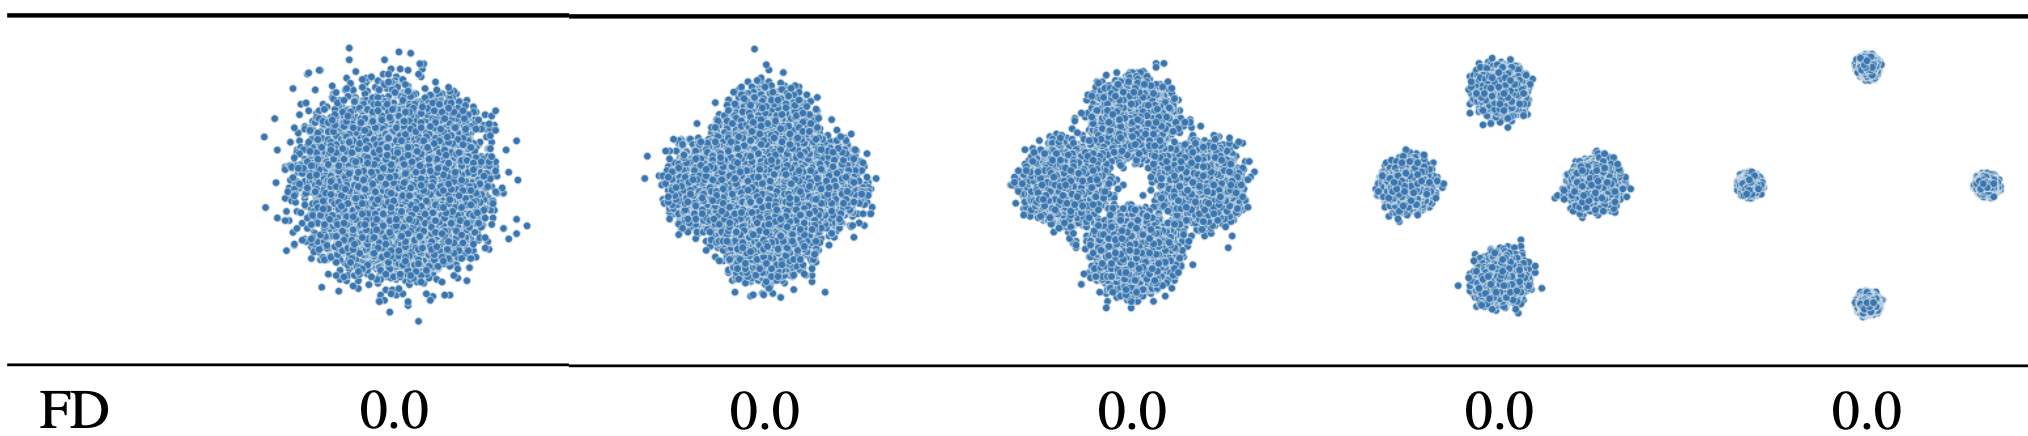
\includegraphics[width=0.95\linewidth]{figs/fid_normal}
		\end{figure}
	\end{block}
\end{frame}
%=======
\begin{frame}{Frechet Inception Distance (FID)}
	\myfootnotewithlink{https://arxiv.org/abs/2401.09603}{Jayasumana S. et al. Rethinking FID: Towards a Better Evaluation Metric for Image Generation, 2024}
	\vspace{-0.4cm}
	\[
		\FID (\pd, \pt) = \| \bmu_{\text{data}} - \bmu_{\btheta}\|^2 + \tr \left[ \bSigma_{\text{data}} + \bSigma_{\btheta} - 2 \left(\bSigma_{\text{data}}^{1/2} \bSigma_{\btheta} \bSigma_{\text{data}}^{1/2} \right)^{1/2} \right]
	\]
	\eqpause
	\vspace{-0.3cm}
	\begin{block}{Drawbacks}
		\begin{itemize}
			\item Depends on the pretrained classification network.
			\item Uses the normality assumption.
			\item May not correlate with human evaluation.
		\end{itemize}
	\end{block}
	\begin{figure}
		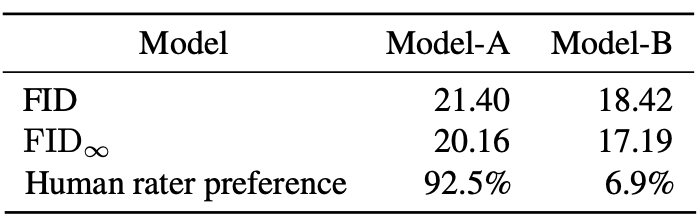
\includegraphics[width=0.7\linewidth]{figs/fid_vs_human_eval}
	\end{figure}
\end{frame}
%=======
\subsection{Precision-Recall}
%=======
\begin{frame}{Precision-Recall}
	\myfootnotewithlink{https://arxiv.org/abs/1904.06991}{Kynkäänniemi T. et al. Improved precision and recall metric for assessing generative models, 2019}
	\vspace{-0.5cm}
	\begin{block}{Desirable Properties for Samples}
		\begin{itemize}
			\item \textbf{Sharpness}: generated samples should possess high visual quality.
			\item \textbf{Diversity}: their variation should match that in the training data.
		\end{itemize}
	\end{block}
	\eqpause
	\vspace{-0.5cm}
	\begin{figure}
		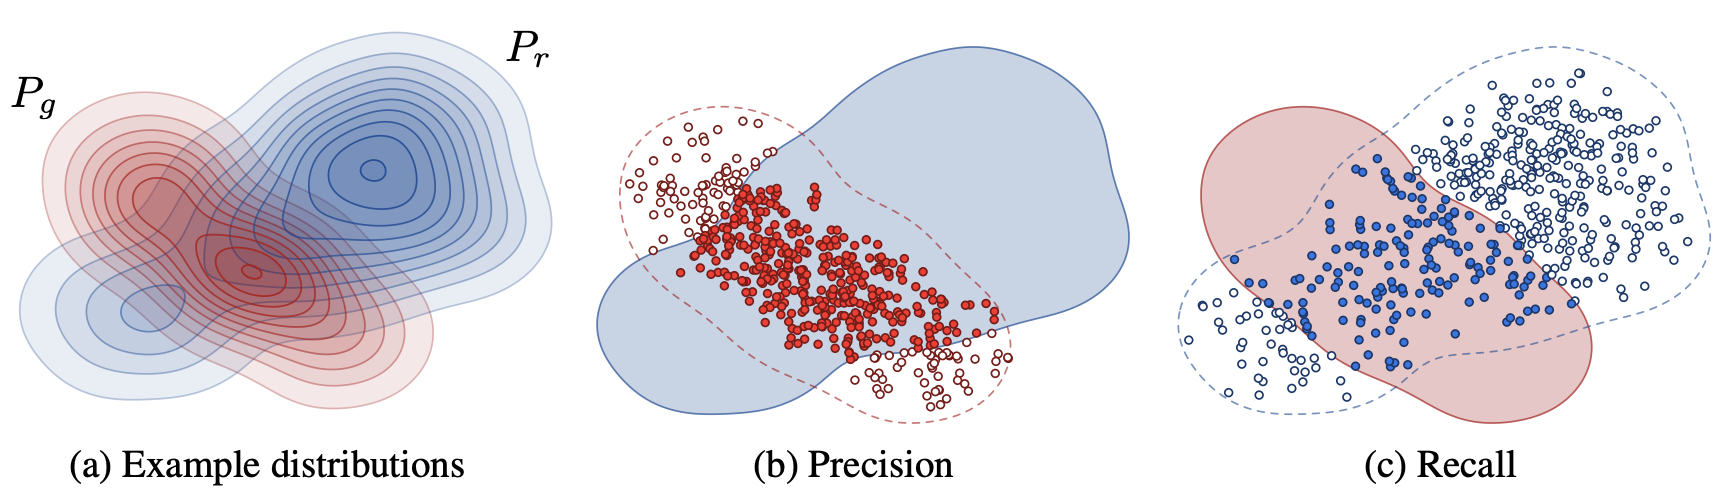
\includegraphics[width=0.9\linewidth]{figs/pr_curve}
	\end{figure}
	\vspace{-0.3cm}
	\begin{itemize}
		\item \textbf{Precision} denotes the fraction of generated images that look realistic.
		\item \textbf{Recall} measures how well the generator covers the training data manifold.
	\end{itemize}
\end{frame}
%=======
\begin{frame}{Precision-Recall}
	\myfootnotewithlink{https://arxiv.org/abs/1904.06991}{Kynkäänniemi T. et al. Improved precision and recall metric for assessing generative models, 2019}
	\vspace{-0.2cm}
	\begin{itemize}
		\item $\cS_{\text{data}} = \{\bx_i\}_{i=1}^{n} \sim \pd(\bx)$ -- real samples;
		\item $\cS_{\btheta} = \{\bx_i\}_{i=1}^{n} \sim \pt(\bx)$ -- generated samples.
	\end{itemize}
	\eqpause
	Define a binary function:
	\vspace{-0.2cm}
	\[
		\bbI(\bx, \cS) =
		\begin{cases}
			1, & \text{if } \exists\ \bx' \in \cS: \| \bx - \bx'\|_2 \leq \| \bx' - \NN_k(\bx', \cS)\|_2; \\
			0, & \text{otherwise.}
		\end{cases}
	\]
	\eqpause
	\vspace{-0.3cm}
	\[
		\text{Pr} (\cS_{\text{data}}, \cS_{\btheta}) = \frac{1}{n} \sum_{\bx \in \cS_{\btheta}} \bbI(\bx, \cS_{\text{data}}); \quad \text{Rec} (\cS_{\text{data}}, \cS_{\btheta}) = \frac{1}{n} \sum_{\bx \in \cS_{\text{data}}} \bbI(\bx, \cS_{\btheta}).
	\]
	\eqpause
	\vspace{-0.6cm}
	\begin{figure}
		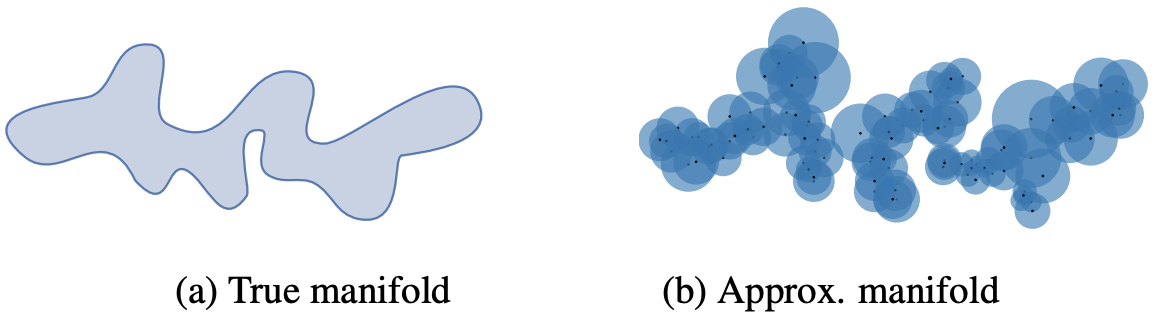
\includegraphics[width=0.75\linewidth]{figs/pr_k_nearest}
	\end{figure}
	\eqpause
	Embed the samples using a pretrained network (as in FID).
\end{frame}
%=======
\begin{frame}{Precision-Recall}
	\myfootnotewithlink{https://arxiv.org/abs/1904.06991}{Kynkäänniemi T. et al. Improved precision and recall metric for assessing generative models, 2019}
	\vspace{-0.3cm}
	\begin{figure}
		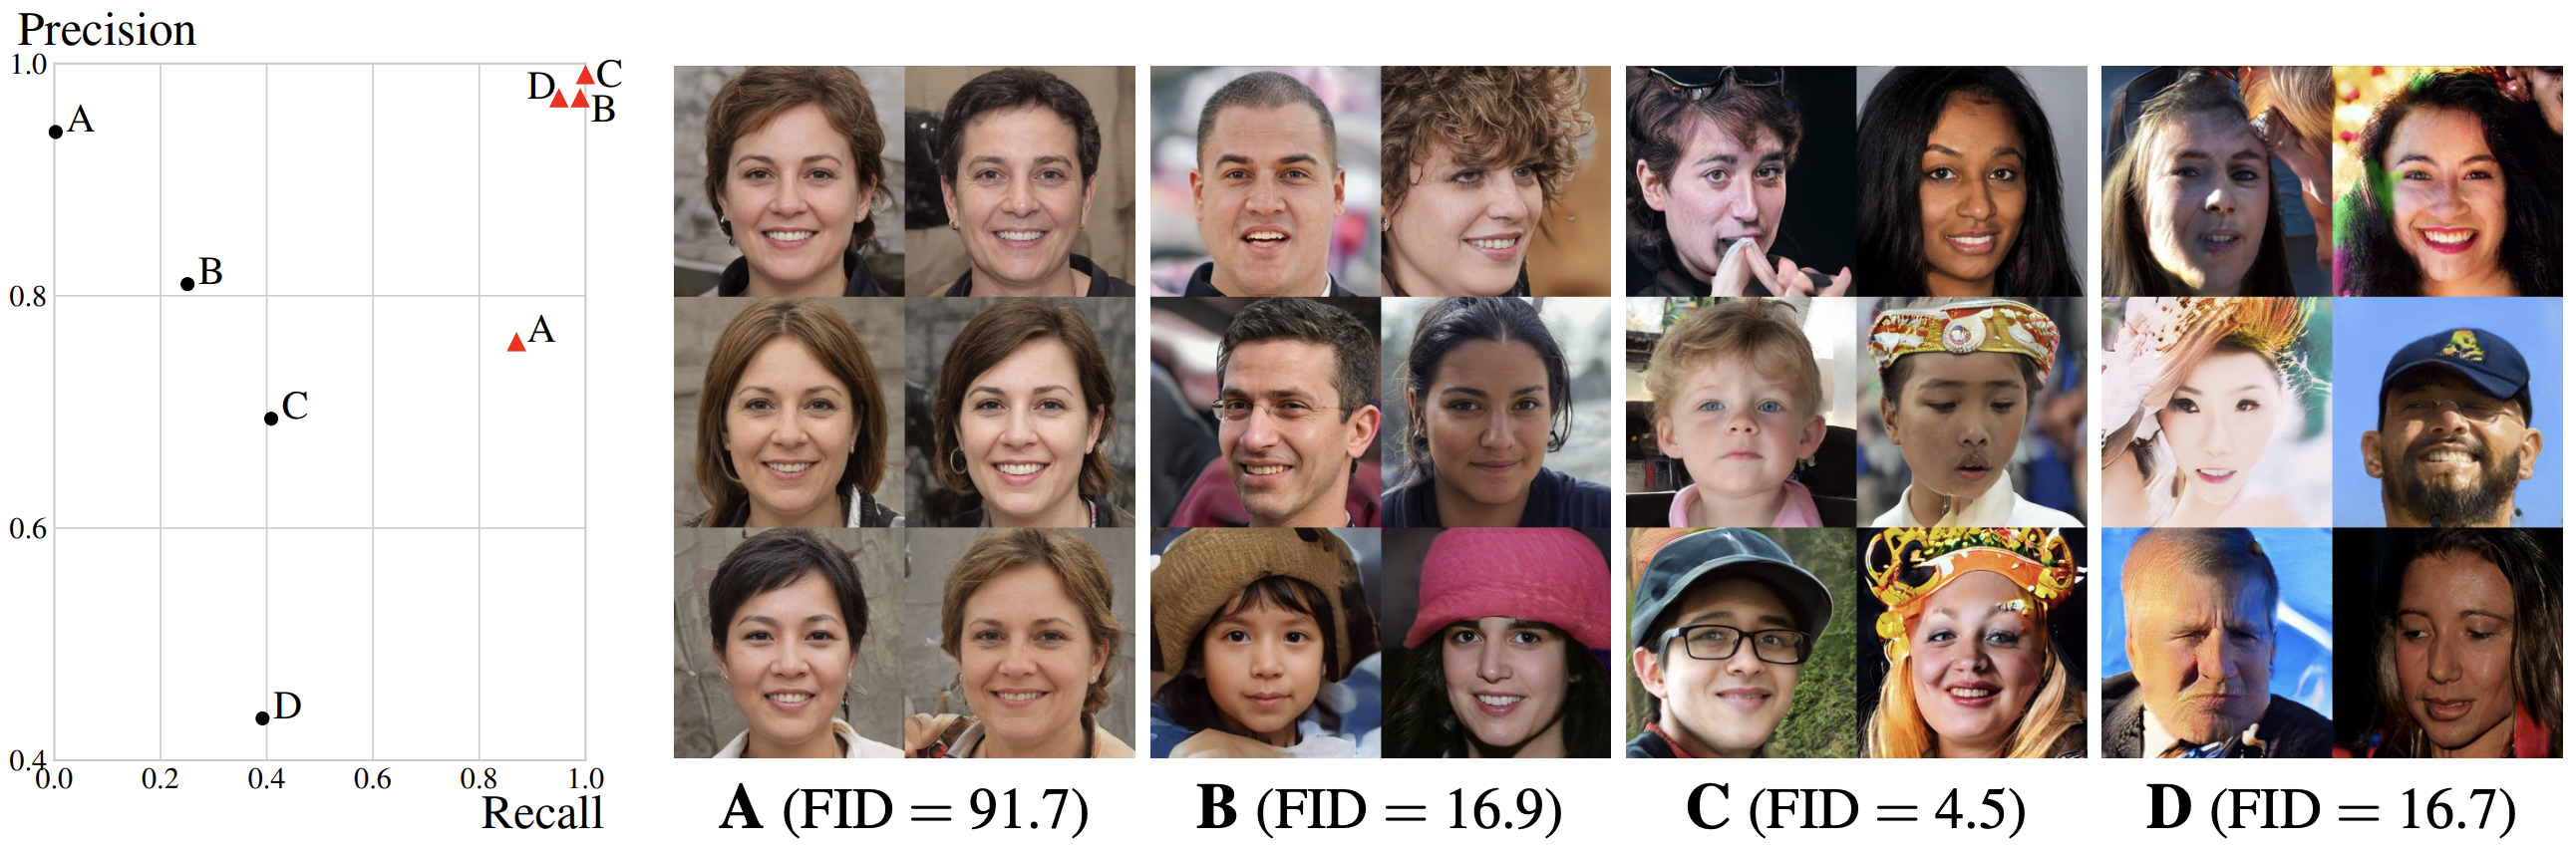
\includegraphics[width=\linewidth]{figs/pr_vs_fid}
	\end{figure}
	\eqpause
	\vspace{-0.3cm}
	\begin{figure}
		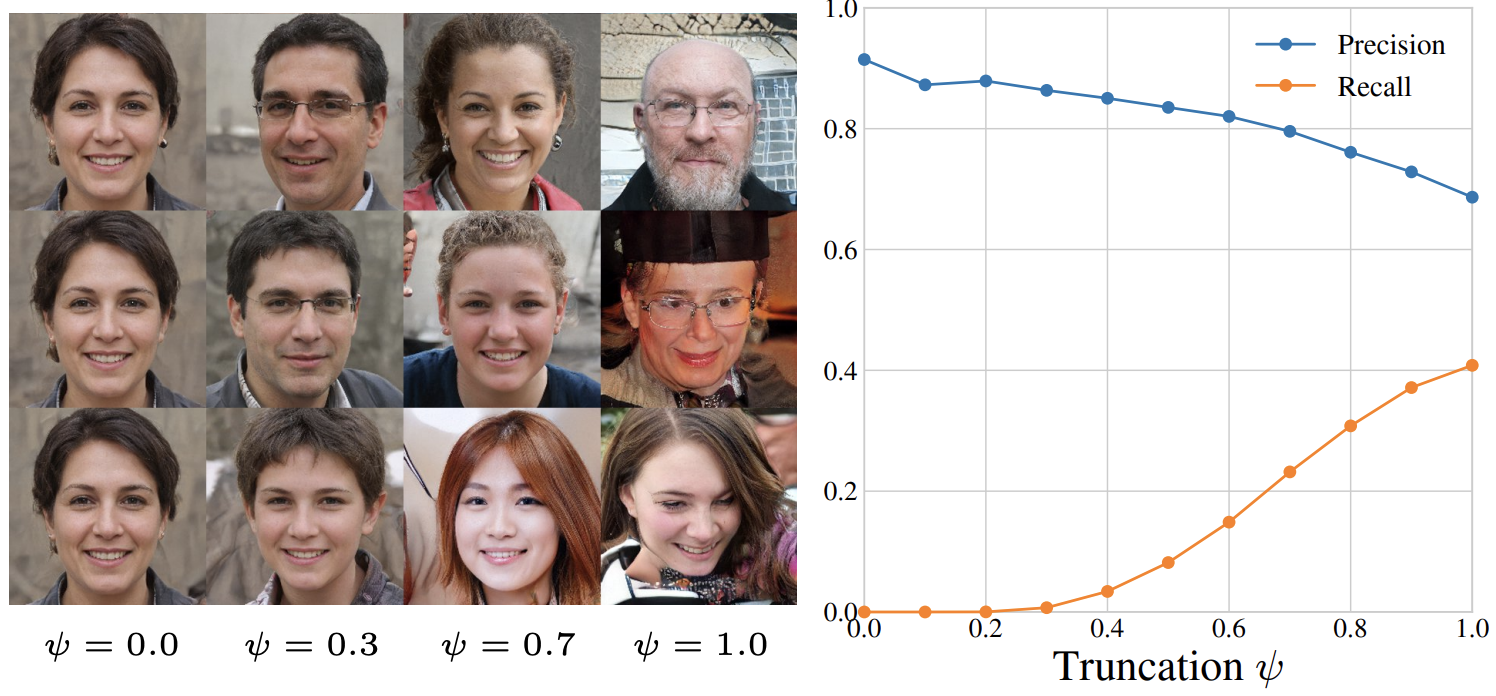
\includegraphics[width=0.75\linewidth]{figs/pr_truncation}
	\end{figure}
\end{frame}
%=======
\subsection{CLIP Score}
%=======
\begin{frame}{CLIP Score}
	\myfootnotewithlink{https://arxiv.org/abs/2103.00020}{Radford A. et al. Learning transferable visual models from natural language supervision, 2021} 
	\vspace{-0.5cm}
	\begin{minipage}{0.5\linewidth}
		\begin{block}{Unconditional Model}
			\begin{figure}
				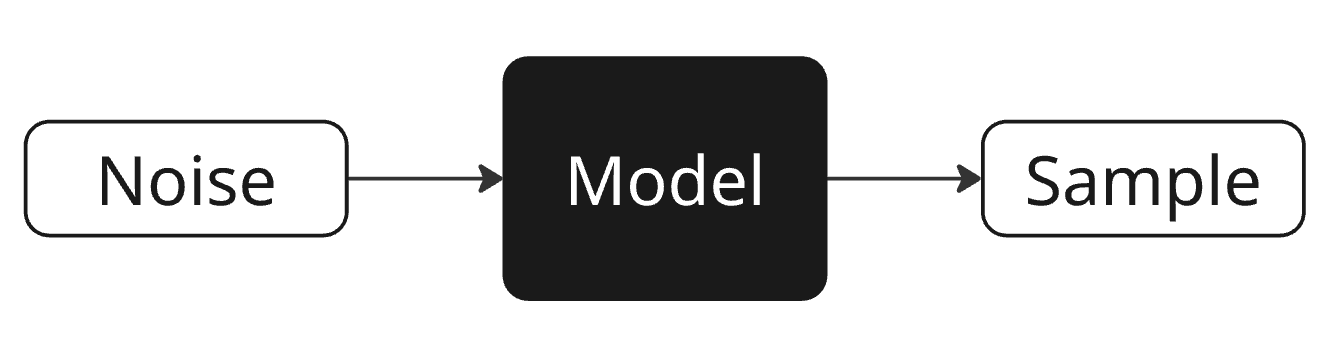
\includegraphics[width=0.95\linewidth]{figs/uncond_model}
			\end{figure}
		\end{block}
		\vspace{0.2cm}
	\end{minipage}%
	\begin{minipage}{0.5\linewidth}
		\begin{block}{Conditional Model}
			\begin{figure}
				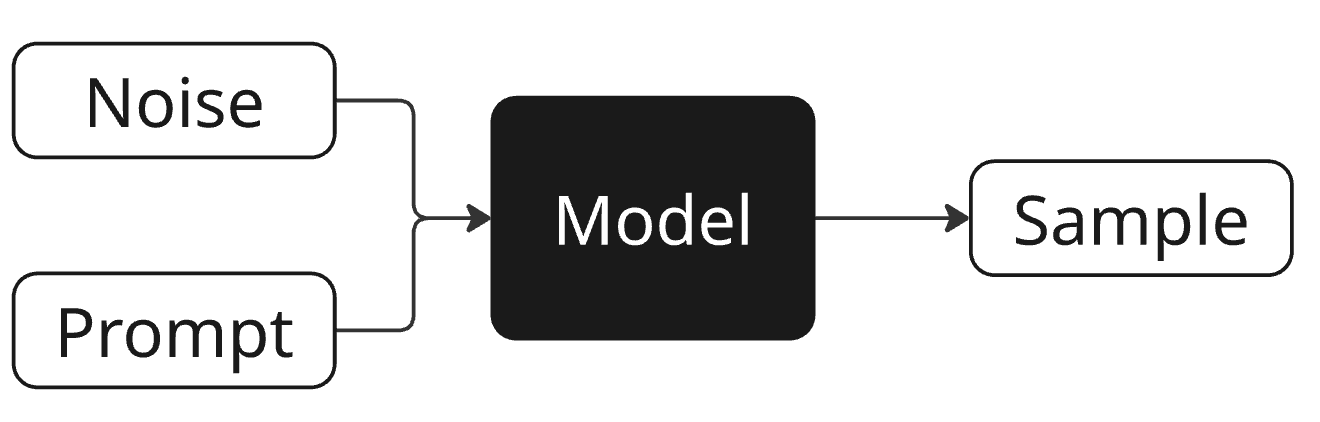
\includegraphics[width=0.95\linewidth]{figs/cond_model}
			\end{figure}
		\end{block}
	\end{minipage}

	\eqpause
	We need a way to measure not only the quality of the generated image, but also how well it's aligned with the prompt.
	\eqpause
	\begin{figure}
		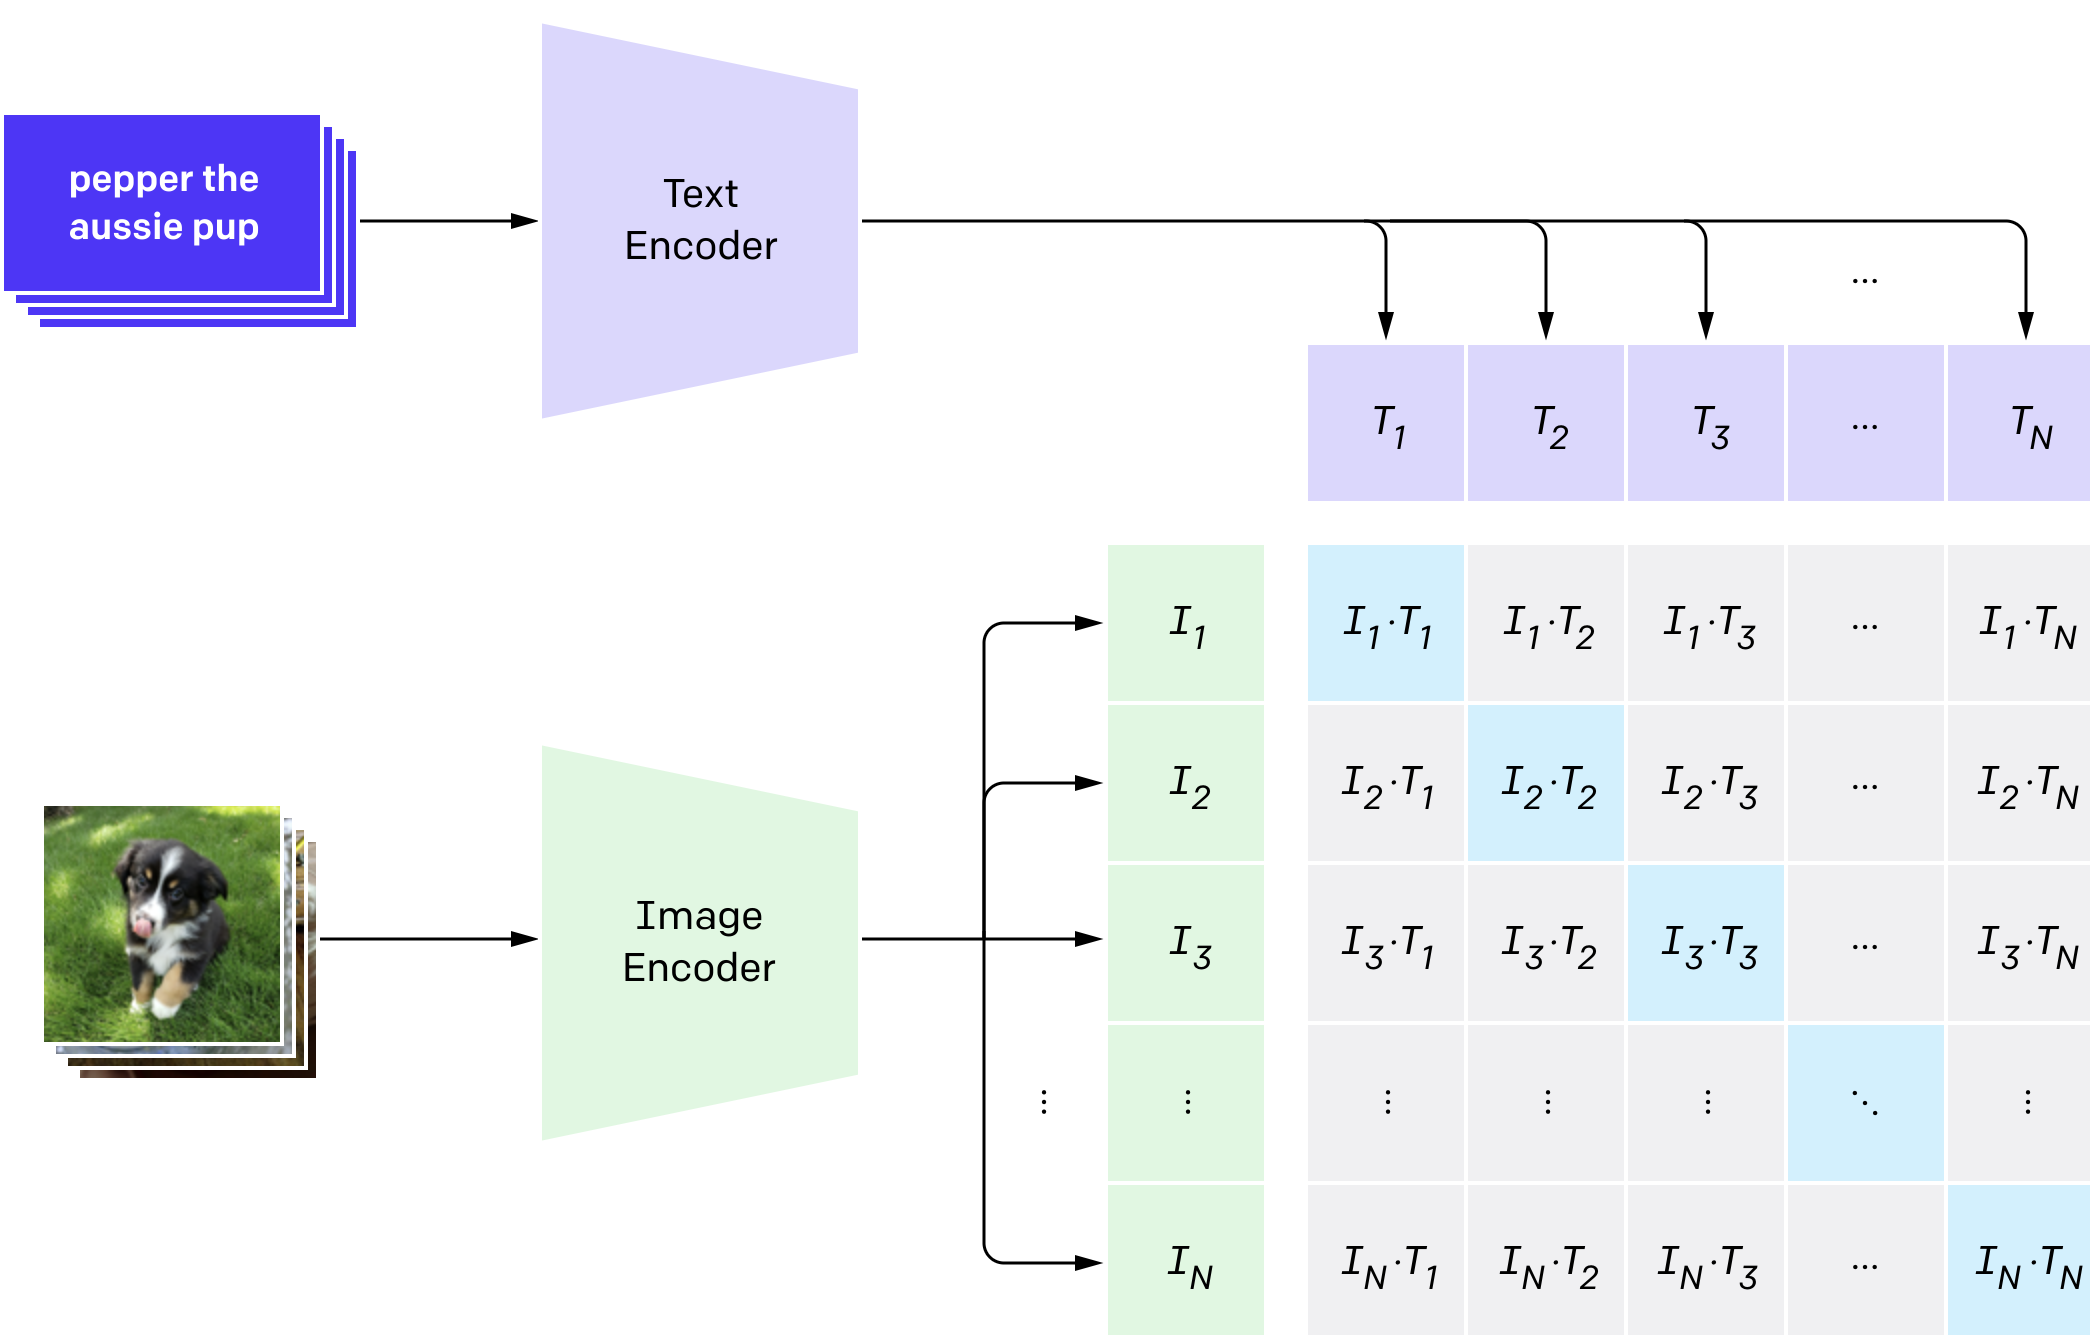
\includegraphics[width=0.6\linewidth]{figs/clip}
	\end{figure}
\end{frame}
%=======
\subsection{Human Eval}
%=======
\begin{frame}{Human Evaluation}
	\myfootnotewithlink{https://ya.ru/ai/art}{YandexART 2.5, 2025} 
	\begin{itemize}
		\item No automated metric is perfect.
		\item The best way to evaluate generative models is by human assessment.
		\item It's important to assess various properties.
	\end{itemize}
	\eqpause
	\begin{figure}
		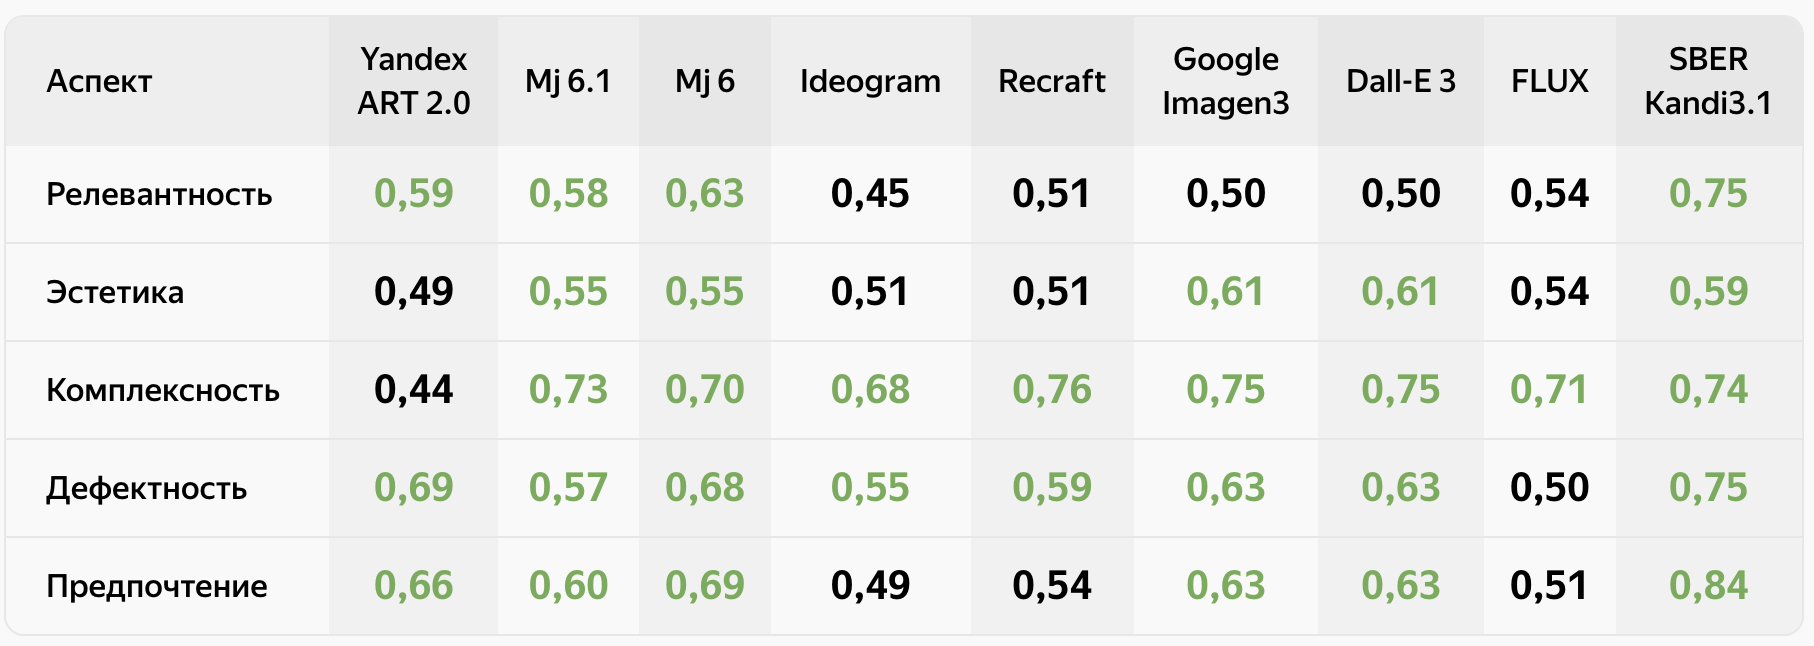
\includegraphics[width=1.0\linewidth]{figs/yaart_2.5}
	\end{figure}
\end{frame}
%=======
\begin{frame}{Summary}
	\begin{itemize}
		\item GANs, in theory, optimize the Jensen-Shannon divergence.
		\vfill
		\item Wasserstein distance works in the case of disjoint data and model distributions (unlike the KL and JS divergences).
		\vfill
		\item Wasserstein GAN uses Kantorovich-Rubinstein duality to enable Monte Carlo estimation of the Wasserstein distance. It enforces the Lipschitz condition on the critic through weight clipping.
		\vfill
		\item FID is the most popular metric for evaluating implicit generative models.
		\vfill
		\item Precision-recall allows for choosing a model that balances sample quality and diversity.
		\vfill
		\item The CLIP score is widely used to measure text-to-image alignment.
		\vfill
		\item The gold standard for evaluating generated image quality is human assessment.
	\end{itemize}
\end{frame}
%=======
\end{document}